\documentclass[10pt, total={6in, 8in}]{extarticle}
% (1) Encoding, Fonts, and Layout
\usepackage[T1]{fontenc}
\usepackage{lmodern}
\usepackage[margin=1in]{geometry}


% (2) Common Packages
\usepackage{amsmath, amssymb, amsthm}
\usepackage{xcolor}
\usepackage{caption}
\usepackage{tikz}
\usepackage{pgfplots}
\pgfplotsset{compat=newest}
\usepackage{etoolbox}
\usepackage{tikz-3dplot}
\tdplotsetmaincoords{75}{120}
\usepackage[inline]{enumitem}
\usepackage{bookmark}
\usepackage{mathtools}
\usepackage{subcaption} % For subfigures
\usepackage[normalem]{ulem} % For better underline commands

% Micro-typography
\usepackage{microtype}

% Patching pgfplots warning
\makeatletter
\patchcmd{\pgfplots@applistXXpushback@smallbuf}{\pgfplots@error}{\pgfplots@warning}{}{}
\makeatother

% (3) tcolorbox and Theorem Libraries
\usepackage{tcolorbox}
\tcbuselibrary{theorems}

% (4) Define Colors
\definecolor{custom_green}{HTML}{a3be8c}
\definecolor{custom_red}{HTML}{dc322f}
\definecolor{custom_blue}{HTML}{268bd2}
\definecolor{custom_purple}{HTML}{b48ead}

\definecolor{base}{HTML}{eceff4}
\definecolor{gray1}{HTML}{e5e9f0}
\definecolor{gray2}{HTML}{d8dee9}
\definecolor{gray3}{HTML}{2e3440}
\pagecolor{base}

% (5) Custom tcolorbox Environments
\newtcolorbox{definitionbox}[1][]{
    title=\textbf{Definition} {#1},
    fonttitle=\bfseries\boldmath,
    arc=0mm,
    bottomtitle=0.5mm,
    boxrule=0mm,
    colbacktitle=gray2,
    colback=gray1,
    coltitle=gray3,
    coltext=gray3,
    left=2.5mm,
    leftrule=1mm,
    rightrule=1mm,
    right=3.5mm,
    toptitle=0.75mm,
    colframe=custom_red,
}

\newtcolorbox{proofbox}{
    title=\textbf{Proof},
    fonttitle=\bfseries\boldmath,
    arc=0mm,
    bottomtitle=0.5mm,
    boxrule=0mm,
    colbacktitle=gray2,
    colback=gray1,
    coltitle=gray3,
    left=2.5mm,
    leftrule=1mm,
    rightrule=1mm,
    right=3.5mm,
    toptitle=0.75mm,
    colframe=custom_blue,
    coltext=gray3,
}

\newtcolorbox{theorembox}[1][]{
    title=\textbf{Theorem} {#1},
    fonttitle=\bfseries\boldmath,
    arc=0mm,
    bottomtitle=0.5mm,
    boxrule=0mm,
    colbacktitle=gray2,
    colback=gray1,
    coltitle=gray3,
    left=2.5mm,
    leftrule=1mm,
    rightrule=1mm,
    right=3.5mm,
    toptitle=0.75mm,
    colframe=custom_green,
    coltext=gray3
}

\newtcolorbox{notebox}{
    title=\textbf{Note},
    fonttitle=\bfseries\boldmath,
    arc=0mm,
    bottomtitle=0.5mm,
    boxrule=0mm,
    colbacktitle=gray2,
    coltitle=gray3,
    left=2.5mm,
    leftrule=1mm,
    rightrule=1mm,
    right=3.5mm,
    toptitle=0.75mm,
    colframe=custom_blue,
    coltext=gray3
}

\newtcolorbox{examplebox}[1][]{
    title=\textbf{Example} {#1},
    fonttitle=\bfseries\boldmath,
    arc=0mm,
    bottomtitle=0.5mm,
    boxrule=0mm,
    colbacktitle=gray2,
    colback=gray1,
    coltitle=gray3,
    left=2.5mm,
    leftrule=1mm,
    rightrule=1mm,
    right=3.5mm,
    toptitle=0.75mm,
    colframe=gray3,
    fontupper=\footnotesize,
    coltext=gray3
}

% (6) Theorem Environments
\theoremstyle{definition}
\newtheorem{definition}{Definition}[section]
\newtheorem{example}[definition]{Example}

\theoremstyle{plain}
\newtheorem{theorem}[definition]{Theorem}

% (7) Hyperlinks
\usepackage{hyperref}
\hypersetup{
    colorlinks=true,    % Use colored text for links
    linkcolor=custom_red,      % Set link text color to red
    pdfborder={0 0 0}   % Remove the default box around links
}

% macros.tex
\newcommand{\intinf}{\int_0^{\infty}} % Integral from 0 to infinity
\newcommand{\diff}[2]{\frac{d#1}{d#2}} % Derivative


\usepackage[svgnames]{xcolor}
\usepackage{listings}
\usepackage{changepage}
\usepackage{geometry}
 \geometry{
 a4paper,
 total={170mm,257mm},
 bottom=20mm,
 top=10mm
 }
\begin{document}

\begin{center}
    Robert Davidson\\
    BSc Mathematics and Computer Science\\[24pt]

    \large
    \textbf{Statistics (ST1112) notes}\\[6pt]
    \small
    Date: \today\\[48pt]
    \small
\end{center}
\begin{abstract}
    \begin{adjustwidth}{1cm}{1cm}
        These notes provide a concise overview of foundational topics in inferential statistics, focusing on how to use sample data to estimate unknown population parameters and assess the strength of evidence against hypothesized values. Beginning with key distinctions between probability (forward calculations from models) and statistics (inference from observed data), the document introduces core definitions—population vs. sample, sampling distributions, and the Central Limit Theorem—to justify the use of normal approximations in many practical settings. \\[2ex]
        Subsequent sections cover confidence intervals, highlighting both $z$-based and $t$-based methods for estimating a population mean (depending on sample size and variance knowledge), and analogous approaches for proportions and counts (including Poisson-based reasoning). The role of transformations and bootstrap procedures is emphasized when normal assumptions are questionable or for robust nonparametric estimation. \\[2ex]
        Readers are then guided through hypothesis testing, from one-sample and two-sample tests for means and proportions to the concepts of significance level ($\alpha$), Type I/II errors, and test power. The discussion extends to chi-squared tests for categorical data, showing how to test goodness-of-fit to hypothesized distributions or independence in contingency tables. \\[2ex]
        Finally, the notes explore methods for quantifying linear relationships between variables, including correlation (Pearson's $r$, Spearman's $\rho$, Kendall's $\tau$) and simple linear regression. Key assumptions, diagnostic checks, and interpretation of regression coefficients, $R^2$, and residual analyses are explained. Throughout, the document underscores the difference between statistical and practical significance, cautioning against over-interpretation of p-values and correlation as evidence of causation.
    \end{adjustwidth}
\end{abstract}

\pagebreak

\scriptsize\tableofcontents\normalsize

\pagebreak

\section{Inferential Statistics - Interval Estimation}
The ultimate goal in statistical inference is to estimate population parameters (like the mean $\mu$) based on sample statistics (like the sample mean $\bar{X}$).
\subsection{Probability vs Statistics}
\begin{itemize}
    \item \textbf{Probability} deals with known underlying processes: one starts with a model (like proportion of red vs. green jelly beans in a jar) and computes probability of specific outcomes
    \item \textbf{Statistics} works in reverse: one observes outcomes (sample data) and attempts to infer the underlying process or population parameters (e.g. proportion of red jellybeans)
\end{itemize}
\subsection{Definitions and Concepts}

\begin{definitionbox}{Population}{}
    A \textbf{population} is the complete set of items (or individuals) of interest.
\end{definitionbox}

\begin{definitionbox}{Sample}{}
    A \textbf{sample} is a subset of that population, intended to represent the population\\

    For example the sample mean $\bar{X}$ is an estimate of the population mean $\mu$.
\end{definitionbox}

\begin{definitionbox}{Population Mean ($\mu$)}{}
    $\mu$ represents the central tendency of a population distribution.
    $$\mu = \frac{1}{N} \sum_{i=1}^{N} x_i$$
    where $N$ is the population size and $x_i$ are the individual values in the population.\\

    $\mu$ is sometimes called the expected value or average.
\end{definitionbox}

\begin{definitionbox}{Population standard deviation ($\sigma$)}{}
    $\sigma$ measures the dispersion or spread of values around the mean in a population.
    $$\sigma = \sqrt{\frac{1}{N} \sum_{i=1}^{N} (x_i - \mu)^2}$$
    where $N$ is the population size and $x_i$ are the individual values in the population.\\
\end{definitionbox}

\begin{conceptbox}{Sampling Variation}{}
    When we take multiple samples from the same population, each sample's mean $\bar{X}$ will be different. This is variability is called \textbf{sampling variation}. \\

    Larger sample sizes tend to reduce this variation, that is as $n$ gros, the sample mean $\bar{X}$ becomes a better estimate of the population mean $\mu$.
\end{conceptbox}
\begin{conceptbox}{Sampling Distributions}{}
    The sample mean itself is a \textbf{random variable} because different samples yield different mean values.\\

    The distribution of all possible sample means (of a given sample size $n$) is called the \textbf{sampling distribution} of the sample mean ($\bar{X}$).
\end{conceptbox}

\begin{definitionbox}{Expected Value of the Sample Mean}{}
    $$E(\bar{X}) = \mu$$
    This means if you averaged all possible sample means, you would get the population mean $\mu$.
\end{definitionbox}
\begin{definitionbox}{Standard Error of the Mean}{}
    $$SE = SD(\bar{X}) = \frac{\sigma}{\sqrt{n}}$$
    where $\sigma$ is the population standard deviation and $n$ is the sample size.\\

    This value is called the \textbf{standard error} of the mean and measures how much the sample mean $\bar{X}$ fluctuates around the population mean $\mu$.
\end{definitionbox}

\begin{definitionbox}{Central Limit Theorem}{}
    $$\bar{X} \sim N\left(\mu, \frac{\sigma^2}{n}\right)$$
    where $\bar{X}$ is the sample mean, $\mu$ is the population mean, and $\sigma$ is the population standard deviation.\\

    The \textbf{Central Limit Theorem} states that the sampling distribution of the sample mean $\bar{X}$ (the distribution of all sample means)  approaches a normal distribution as the sample size $n$ increases, \textbf{regardless of the shape of the population distribution.}\\

    This means that for large enough sample sizes, we can use the normal distribution to make inferences about the population mean $\mu$. \\

    \textbf{Practically}, many apply the rule of thumb $n \geq 30$ to treat $\bar{X}$ as normally distributed.
\end{definitionbox}


\begin{definitionbox}{Unbiased Estimators}{}
    We say a statistic $T$ is an \textbf{unbiased estimator} of a population parameter $\theta$,  if $E(T) = \theta$.\\

    For example, the sample mean $\bar{X}$ is an unbiased estimator of the population mean $\mu$ because $E(\bar{X}) = \mu$.\\

    The sample standard deviation $s$ (using Bessel's correction, dividing by multiplying by $\frac{1}{n-1}$ rather than $\frac{1}{N}$) is an unbiased estimator of the population standard deviation $\sigma$.
\end{definitionbox}

\subsection{Example}
\begin{examplebox}{Weekly rent}{}
    If a population mean rent is $\mu = 225$, with $\sigma = 25$ for a population sample size $n = 30$, the sample distribution of the sample mean is approximately:
    $$\bar{X} \sim N\left(225, \frac{25^2}{30}\right)$$
    This lets us compute probabilities for specific sample mean ranges using the normal distribution (e.g. $P(\bar{X} < 220)$).
\end{examplebox}
\subsection{Recap}
A \textbf{sample statistic} (e.g. the sample mean $\bar{X}$) varies from one sample to another. Understanding this variation (and quantifying it via the standard error) is crucial for knowing how precise (or imprecise) an estimate really is. \\[2ex]
If we have a large sample size $n$ from a population with mean $\mu$ and standard deviation $\sigma$, then our sample distribution of the sample mean $\bar{X}$ is approximately normal:
$$\bar{X} \sim N\left(\mu, \frac{\sigma^2}{n}\right)$$
In practice, for $n \geq 30$, $\bar{X}$ can be treated as normally distributed even if the original population is not strictly normal.

\section{Confidence Intervals}

\subsection{Confidence Intervals}
\begin{conceptbox}{Why confidence intervals?}{}
    Why do we need confidence intervals, instead of a single point estimate, like the sample mean $\bar{X}$? \\

    A confidence interval provides a range of plausible values for the population parameter (e.g. $\mu$) based on the sample data. \\

    \textbf{Analogy:}  Using a single point estimate is like trying to catch a fish wih a spear; your aim may not be perfect. Using a confidence interval is like using a net; we have a better chance of "catching" (capturing) the true population parameter.
\end{conceptbox}
\begin{definitionbox}{Confidence Interval}{}
    $$\bar{X} \pm (\text{critical value}) \times SE(\bar{X})$$
    where $SE(\bar{X}) = \frac{\sigma}{\sqrt{n}}$ is the standard error of the sample mean, $\pm$ is the margin of error. \\
    The general formula for a desired confidence level 100(1- $\alpha$)\% is:
    $$\bar{X} \pm z_{\alpha/2} \times \frac{\sigma}{\sqrt{n}}$$
    where $z_{\alpha/2}$ is the critical value from the standard normal distribution.
\end{definitionbox}
\noindent\textbf{Interpretation}: \\
If we repeat the sampling process many times and construct confidence intervals from each sample, then approximately $100 \times (1 - \alpha)\%$ of those intervals will contain the true population parameter $\mu$.\\
In other words, you do not say \emph{"there is a 95\% chance that $\mu$ lies in my interval"}. Rather we say, \textbf{"on repeated sampling 95\% of such intervals will contain the true population mean $\mu$."}


\begin{definitionbox}{Critical Values}{}
    The \textbf{critical value} is a z-score that corresponds to the desired confidence level. \\[2ex]
    For example, for a 95\% confidence level, the critical value is $Z_{\alpha/2} = 1.96$ (where $\alpha = 0.05$).
    This means that 95\% of the area under the normal curve lies within $1.96$ standard deviations of the mean. \\[2ex]
    \begin{center}
        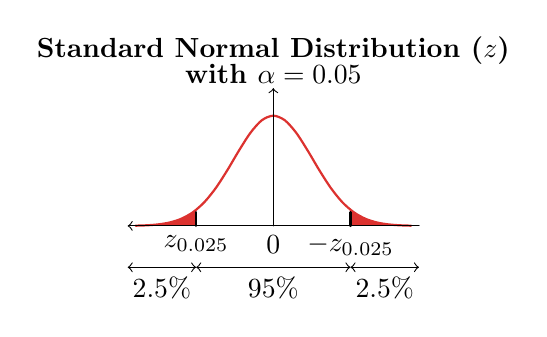
\begin{tikzpicture}[
                domain=-1:1,
                xscale=-0.5,
                yscale=3.5,
                smooth,
                line cap=round,
                line join=round,
            ]
            % Define critical z values
            \def\zcrit{1.96}

            % Fill left tail area (2.5%)
            \fill[custom_red] (-3.5,0) -- plot[domain=-3.5:-\zcrit] (\x, {0.4*exp(-(\x)^2/2)}) -- (-\zcrit,0) -- cycle;

            % Fill right tail area (2.5%)
            \fill[custom_red] (3.5,0) -- plot[domain=3.5:\zcrit] (\x, {0.4*exp(-(\x)^2/2)}) -- (\zcrit,0) -- cycle;

            % Draw the normal distribution curve
            \draw[thick, custom_red] plot[domain=-3.5:3.5] (\x, {0.4*exp(-(\x)^2/2)});

            % Mark the critical values
            \draw[thick] (-\zcrit,0) -- (-\zcrit,0.05);
            \node[below] at (-\zcrit,0) {$-z_{0.025}$};
            \draw[thick] (\zcrit,0) -- (\zcrit,0.05);
            \node[below] at (\zcrit,0) {$z_{0.025}$};

            \draw[<->] (-\zcrit, -0.15) -- (\zcrit, -0.15) node[midway, below] {$95\%$};
            \draw[<->] (-\zcrit, -0.15) -- (-3.7, -0.15) node[midway, below] {$2.5\%$};
            \draw[<->] (\zcrit, -0.15) -- (3.7, -0.15) node[midway, below] {$2.5\%$};


            % Draw horizontal axis
            \draw[->] (-3.7,0) -- (3.7,0) node[right] {};
            % Draw vertical axis
            \draw[->] (0,0) -- (0,0.5) node[above] {};
            % Mark the center
            \node[below] at (0,0) {$0$};
            % Title
            \node[above] at (0,0.55) {\textbf{Standard Normal Distribution ($z$)}};
            \node at (0,0.55) {\textbf{with $\alpha = 0.05$}};
        \end{tikzpicture}
    \end{center}
\end{definitionbox}

\begin{examplebox}{Find crtitical value for the 95\% CI}{}
    For a confidence interval of 95\%, we want to find the z-score that leaves 2.5\% in each tail of the normal distribution.\\
    We want to find the $z$-value where the cumulative area (from the left up to that $z-score$) is $1 - 0.025 = 0.975$.\\
    We look in the $z$-tables for the value closest to $0.975$ and read the row and column headers to find the $z$-value.\\
    The $z$-value is $1.96$.\\
\end{examplebox}

\begin{examplebox}{Find the 95\% confidence interval for the population mean $\mu$ given}{}
    A dataset of 103 students, of whom 71 pay rent, was used to estimate the average weekly rent $\mu$.
    \begin{itemize}
        \item \textbf{Point estimate}: the sample mean $\bar{X} \approx 546.239$.
        \item \textbf{Sample standard deviation}: $s \approx 187.862$.
        \item \textbf{Sample size}: $n = 71$.
    \end{itemize}
    Confidence Interval is given by:
    $$\bar{X} \pm z_{\alpha/2} \times \frac{s}{\sqrt{n}}\Rightarrow 546.239 \pm 1.96 \times \frac{187.862}{\sqrt{71}}$$
    where $z_{\alpha/2} = 1.96$ for a 95\% confidence level.The resulting confidence interval is:
    $$(502.541, 589.938)$$
    \textbf{Interpretation}: We are 95\% confident that the true mean weekly rent for all NUI Galway students (population) is roughly 503 to 590 euros.
\end{examplebox}
\subsection{Higher Confidence Levels means Wider Intervals}
\begin{itemize}
    \item To achieve a \textbf{higher confidence level}, we need to increase the critical value $z_{\alpha/2}$, which in turn increases the margin of error.
    \item This results in a wider confidence interval, which means we are more certain that the true population parameter lies within that interval.
    \item Conversely a \textbf{lower confidence level} results in a smaller critical value, leading to a narrower confidence interval.
\end{itemize}

\subsection{t-Distribution}
\begin{conceptbox}{Why the $t-$distribution}{}
    When the sample size is small ($n < 30$) and the population standard deviation $\sigma$ is unknown, simply substituting the sample standard deviation $s$ no longer suffices because the standard error is itself estimated with more uncertainty.\\[2ex]
    The $\textbf{t-distributution has thicker}$ tails than the normal distributution. This extra "fatness" in the tails accounts for the additional uncertainty in using $s$ instead of $\sigma$.
    \begin{center}
        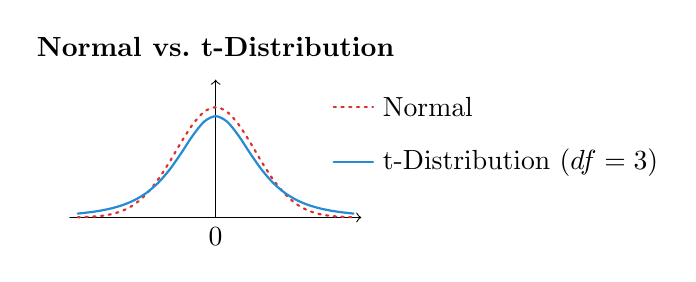
\begin{tikzpicture}[
                domain=-3.5:3.5,
                xscale=0.5,
                yscale=3.5,
                smooth,
                line cap=round,
                line join=round
            ]
            % Draw axes
            \draw[->] (-3.7,0) -- (3.7,0) node[right] {$$};
            \draw[->] (0,0) -- (0,0.5) node[above] {$$};
            \node[below] at (0,0) {$0$};

            % Plot the Normal Distribution (dotted red)
            \draw[dotted, thick, custom_red] plot (\x, {0.4*exp(-(\x)^2/2)});

            % Plot the t-Distribution (solid blue) for df = 5.
            % The t-density: f(t) = (8/(3*pi*sqrt(5)))*(1+t^2/5)^(-3)
            \draw[thick, custom_blue] plot (\x, {(2/(3.14159*sqrt(3)))*((1+(\x)^2/3)^(-2))});

            % Title and legend
            \node[above] at (0,0.55) {\textbf{Normal vs.\ t-Distribution}};

            % Legend (placed at the top-right)
            \begin{scope}[shift={(3,0.4)}]
                \draw[dotted, thick, custom_red] (0,0) -- (1,0);
                \node[right] at (1,0) {Normal};
                \draw[thick, custom_blue] (0,-0.2) -- (1,-0.2);
                \node[right] at (1,-0.2) {t-Distribution ($df=3$)};
            \end{scope}
        \end{tikzpicture}
    \end{center}
\end{conceptbox}

\begin{conceptbox}{Degrees of Freedom (df)}{}
    A t-distribution is characterized by its degrees of freedom, where
    $$df = n - 1 \quad \text{for a sample mean}$$
    As the sample size $n$ increases, the t-distribution approaches the standard normal distribution.\\
    For example, for $n = 30$, $df = 29$ and the t-distribution is very close to the normal distribution.\\
\end{conceptbox}

\begin{definitionbox}{Confidence Intervals (t-based)}{}
    $$\bar{X} \pm t_{\alpha/2, df} \times \frac{s}{\sqrt{n}}$$
    where $t_{\alpha/2, df}$ is the critical value from the t-distribution with $df = n - 1$ degrees of freedom - or from a function like \texttt{qt()} in R.\\

    \textbf{Assumption}: The population itself should be approximately normally distributed when using t-based methods for small sample sizes.
\end{definitionbox}

\begin{examplebox}{Finding t-critical values}{}
    Find the critical value for a 95\% confidence interval with $n = 12$ (so $df = 11$).\\
    We look for the row associated with $df = 11$ and the column associated with $\alpha/2 = 0.025$.\\
    The critical value is:
    $$t_{0.025, 11} \approx 2.201$$
\end{examplebox}

\subsection{CI with large $n$, and $sigma$ unknown}
The $z$-based critical interval is given as:
$$\bar{X} \pm z_{\alpha/2} \times \frac{\sigma}{\sqrt{n}}$$
where $z_{\alpha/2}$ is the critical value from the standard normal distribution.
However, if the population standard deviation $\sigma$ is unknown, we can use the sample standard deviation $s$ as an estimate.\\
This gives us the following confidence interval:
$$\bar{X} \pm z_{\alpha/2} \times \frac{s}{\sqrt{n}}$$
\textbf{Interpretation}: around 95\% of all possible 95\% confidence intervals will contain the true population mean $\mu$. We can visualize that if we drew many repeated samples, sample means will form an overlapping $\mu$ and a small fraction will not.

\subsection{CI with small $\boldsymbol{n}$, and $\boldsymbol{\sigma}$ unknown}
If the sample size is small ($n < 30$) and the population standard deviation $\sigma$ is unknown, we use the t-distribution to construct the confidence interval. This gives us the following confidence interval:
$$\bar{X} \pm t_{\alpha/2, df} \times \frac{s}{\sqrt{n}}$$
where $t_{\alpha/2, df}$ is the critical value from the t-distribution with $df = n - 1$ degrees of freedom.\\
\textbf{Interpretation}: around 95\% of all possible 95\% confidence intervals will contain the true population mean $\mu$. We can visualize that if we drew many repeated samples, sample means will form an overlapping $\mu$ and a small fraction will not.

\begin{examplebox}{Turin Shroud}{}
    A historical cloth's age was tested by carbon dating on 12 pieces ($n = 12$). The sample mean was $x \approx 1261 \ AD$ and the sample standard deviation was $s \approx 61.2 \ AD$. Find the 95\% confidence interval for the population mean age of the cloth. \\[2ex]
    The standard error is given by:
    $$SE = \frac{s}{\sqrt{n}} = \frac{61.2}{\sqrt{12}} \approx 17.67$$
    For a 95\% confidence interval with $n-1 = 11$ degrees of freedom, the critical value is $t_{0.025, 11} \approx 2.201$.\\
    The confidence interval is given by:
    $$\bar{X} \pm t_{\alpha/2, df} \times SE = 1261 \pm 2.201 \times 17.67$$
    The resulting confidence interval is:
    $$(1222, 1300)$$
    \textbf{Interpretation}: The cloth's true average carbon-dated age is plausibly within about 1222-1300 AD. This range casts doubt on claims that the cloth dates from centuries earlier.
\end{examplebox}
\begin{examplebox}{Unathorized Computer Acess}{}
    Find 95\% CI given:
    \begin{itemize}
        \item \textbf{Data}: 18 times between keystrokes
        \item \textbf{Sample mean}: $\bar{X} = 0.29$ seconds
        \item Sample standard deviation: $s = 0.0074$ seconds
    \end{itemize}
    $$n  = 18 \Rightarrow df = 17$$
    For a 95\% confidence interval with $n-1 = 18$ degrees of freedom, the critical value is $t_{0.025, 17} \approx 1.740$.\\
    The resulting confidence interval is:
    $$(0.2532, 0.3268)$$
    \textbf{Interpretation}: We are 95\% confident that the true mean time between keystrokes is between 0.2532 and 0.3268 seconds.
\end{examplebox}
\section{Transformations and the Bootstrap.}
\subsection{When normality is questionable}
Recall that for small $n$, the t-distribution-based confidence interval requires data to be approximately normally distributed in the population. But many real datasets violate this assumption. - e.g. skewed data, heavily tailed data etc. \\[2ex]
\noindent Two broad remedies exist:
\begin{itemize}
    \item \textbf{Data transformation}: Apply a mathematical transformation to make the data more symmetric or bell shape (e.g.log-transformation). Then use t-based or z-based methods on the transformed scale.
    \item \textbf{Non-parametric methods}: Rely less on strict distributional assumptions. The bootstrap is a common and versatile non-parametric method approach to estimating confidence intervals and sampling variability.
\end{itemize}

\subsection{Data Transformations}
\textbf{Purpose}:
\begin{itemize}
    \item If the data has a strongly skewed or otherwise non-normal distribution, applying a suitable transformation (e.g. $\log(x)$, $\sqrt{x}$) can help to make the data more symmetric and bell-shaped.
    \item After the transformation, we can apply t-based or z-based methods can be applied more safely.
\end{itemize}
\textbf{Cautions}:
\begin{itemize}
    \item Finding the right transformation can be tricky; sometimes no simple transformation works well.
    \item Interpretation of results becomes more complex; if you compute a CI for the transformed mean, you must convert (e.g. exponentiate) the results back to the original scale.
    \item Despite these challenges, transformation often prove very useful in practice.
\end{itemize}

\subsection{The Bootstrap}
\textbf{Motivation}:
\begin{itemize}
    \item Bootstrap methods do not require normality assumptions or a large $n$. They rely on the principle that the observed sample can serve as a reasonable proxy for the populations shape.
    \item By resampling with replacement from the original sample (many times), one creates a "bootstrap distribution" that mimics the statistic (e.g. mean, median) of interest.
    \item This bootstrap distribution is then used to estimate hpw the statistic varies, allowing for confidence interval construction and hypothesis testing without explicit formulas.
\end{itemize}
\textbf{Basic Steps (Bootstrap Scheme)}
\begin{enumerate}
    \item \textbf{Resample with replacement}: Take a bootstrap sample of the same size $n$ as the original dataset, but drawn from the dataset with replacement.
    \item \textbf{Calculate Bootstrap statistic}: Compute the same summary measure of interest (e.g. mean, median) on the bootstrap sample.
    \item \textbf{Repeat}: Repeat steps (1) and (2) many times (e.g. 1000 times) to create a distribution of the bootstrap statistic.
    \item \textbf{Construct CI}: The bootstrap distribution of the resampled statistics can be used to determine the middle 95\% (or chosen confidence level) as the CI bounds.
\end{enumerate}


\textbf{Advantages}:
\begin{itemize}
    \item Works for all kinds of statistics (mean, median, proportion, regression coefficients, etc.) even when no closed-form CI exists.
    \item Far fewer assumptions about the underlying population distribution.
\end{itemize}
\textbf{Disadvantages}:
\begin{itemize}
    \item Computationally intensive; requires many resamples (e.g. 1000) to get a good approximation.
    \item Requires the sample itself to be a good representation of the population; if the sample is biased, the bootstrap may not work well.
\end{itemize}
\section{Confidence Intervals for Population Proportions and Counts}
\subsection*{Recap: Confidence Intervals for a Population Mean}

\begin{itemize}
    \item A \textbf{Confidence interval (CI)} provides a range of plausible values for a population parameter
    \item For a large sample ($n \geq 30$) or a known $\sigma$, we often use a z-based interval:
          $$\bar{X} \pm z_{\alpha/2} \times \frac{\sigma}{\sqrt{n}}$$
          or replacing $\sigma$ with $s$ if $\sigma$ is unknown.
    \item For a small sample ($n < 30$) and unknown $\sigma$, we use a t-based interval:
          $$\bar{X} \pm t_{\alpha/2, df} \times \frac{s}{\sqrt{n}}$$
          where $df = n - 1$. Provided the population is approximately normal.
    \item If normality is questionable, we may use transformations or bootstrapping.
\end{itemize}

\subsection{Proportions}

\begin{definitionbox}{Proportion}{}
    The \textbf{proportion} is a way to express the frequency of a specific outcome (labeled as “success”) relative to the total number of trials or observations.
    $$p = \frac{X}{n}$$
    where $p$ is the proportion, $X$ is the number of successes, and $n$ is the total number of trials.
\end{definitionbox}

\begin{conceptbox}{Why proportions?}{}
    Many outcomes are binary or categorical with two possible outcomes (e.g. success/failure, yes/no). Examples:
    \begin{itemize}
        \item Whether a student has a part-time job
        \item Whether a business has fallen victim to a scam
    \end{itemize}
    In such cases, we often estimate a population proportion $\pi$ of successes rather than a mean $\mu$.
\end{conceptbox}

\subsubsection{Binomial Distribution}
\begin{conceptbox}{Bernoulli Trials}{}
    When we repeat an experiment or observation, each trial is assumed to be independent and has two possible outcomes. If each trial has a probability of $\pi$ success, these trials are called \textbf{Bernoulli trials}.
\end{conceptbox}

\noindent If we perform $n$ independent Bernoulli trials, the number of successes $X$ follows a \textbf{binomial distribution} with $n$, the number of trials and $\pi$,the probability of success on each trial.
$$X \sim B(n, \pi)$$
This tells us how likely we are to observe a certain number of successes in $n$ trials.\\[2ex]
\textbf{Link to Proportion}: \\
The sample proportion $p$ is just the normalized version of $X$, calculated by $p = \frac{X}{n}$. It provides a direct, interpretable measure of success rate in the sample.

\subsubsection{Normal Approximation of the Sample Proportion}
\textbf{When is the normal approximation valid?}\\
The approximation of the distribution of $p$ by a normal distribution is valid when both of the following conditions are met:
$$n\pi \geq 5 \quad \text{and} \quad n(1 - \pi) \geq 5$$
These conditions ensure there are enough successes and failures for the approximation to hold. \\[2ex]
\textbf{How does it work?}
Since $X$ is binomially distributed, its mean is $n\pi$ and its variance is $n\pi(1 - \pi)$. When we convert $X$ into the proportion $p$, the mean and variance transform as follows:
\begin{itemize}
    \item Mean of $p$: $E(p) = \frac{E(X)}{n} = \pi$
    \item Variance of $p$: $Var(p) = \frac{Var(X)}{n^2} = \frac{\pi(1 - \pi)}{n}$
\end{itemize}
For large $n$ (above conditions), the distribution of $p$ can be approximated by a normal distribution:
$$p \sim N\left(\pi, \frac{\pi(1 - \pi)}{n}\right)$$\\
\textbf{Interpretation}: \\
This approximation means if we were to make many samples of size $n$, the distribution of the same proportions would cluster around the true proportion, $\pi$, with variability decreasing as the sample size $n$ increases. This normality is what allows statisticians to construct confidence intervals and perform hypothesis tests on population proportions.
\subsubsection{Confidence Intervals for Proportion $\pi$}
\begin{definitionbox}{Confidence Interval for Proportion}{}
    For a large sample size, i.e.:
    $$np \geq 5 \quad\text{and} \quad n(1-p) \geq 5$$
    a 95\% C.I for the population proportion $\pi$ is given by:
    $$p \pm z_{\alpha/2} \times \sqrt{\frac{p(1 - p)}{n}}$$
    where:
    \begin{itemize}
        \item $p$ is the sample proportion (e.g. $\frac{X}{n}$)
        \item $z_{\alpha/2}$ is the critical value from the standard normal distribution (e.g. $1.96$ for 95\% confidence)
        \item The quantity under the square root is the standard error of the sample proportion.
    \end{itemize}
\end{definitionbox}



\begin{examplebox}{Financial Scams}{}
    A survey of $n=80$ small businesses found that $X = 16$ had fallen victim to a financial scam. Find the 95\% confidence that all small businesses have fallen victim to this scam. \\[2ex]

    \begin{itemize}
        \item Sample proportion: $p = \frac{X}{n} = \frac{16}{80} = 0.20$
        \item Standard Error = $SE = \sqrt{\frac{p(1 - p)}{n}} = \sqrt{\frac{0.20(1 - 0.20)}{80}} = \sqrt{\frac{0.20 \times 0.80}{80}} \approx 0.05$
        \item For a 95\% confidence interval $\alpha = 0.05, z_{\alpha/2} = 1.96$.
    \end{itemize}
    The 95\% confidence interval is given by:
    $$p \pm z_{\alpha/2} \times SE = 0.20 \pm 1.96 \times 0.05$$
    The resulting confidence interval is:
    $$\approx (0.10, 0.30)$$
    \textbf{Interpretation}: We are 95\% confident that between 10\% and 30\% of all small businesses have fallen victim to this scam.
\end{examplebox}
\begin{conceptbox}{Proportion CI Test IN R}{}
    The function \texttt{prop.test(x, n, conf.level, correct=False)}  gives a confidence interval for a proportion.
\end{conceptbox}

\subsubsection{Maximizing the Standard Error}
The standard error for a proportion $p$ is given by:
$$SE = \sqrt{\frac{p(1 - p)}{n}}$$
This maximizes at $p = 0.5$. Thus the worst-case margin of error for a 95\% confidence interval is:
$$\approx \pm 2 \times \sqrt{\frac{0.5\times0.5}{n}} = \pm \frac{1}{\sqrt{n}}$$
\textbf{Rule of thumb}: for $n = 1000$, the margin of error is about $1/\sqrt{1000} \approx 0.03$, i.e. 3\% error.
\subsection{Confidence Intervals for Counts}
\subsubsection{Possion Setup}
A count variable $X$, over a fixed interval (e.g. "number of emails per day") often follows a \textbf{Poisson} distribution. with parameter $\lambda$.  \\
Recall $X \sim Poisson(\lambda)$ implies $E(X) = \lambda$ and $Var(X) = \lambda$.
\subsubsection{Central Limit Theorem Approximation}
\begin{definitionbox}{CLT for Poisson}{}
    For large enough $\lambda$, the Central Limit Theorem, implies the sample mean of a Poisson variable is approximately normally distributed:
    $$X \sim N\left(\lambda, \frac{\lambda}{n}\right)$$
    If we have $n$ observations of some Poisson process, the overall mean $\bar{\lambda}$ is used to estimate the population mean $\lambda$. \\[2ex]
    $$\textbf{Criteria}: \quad n\lambda \geq 50$$
\end{definitionbox}

\begin{examplebox}{Emails per Day}{}
    Given a sample of $n=64$ students with a mean of $\bar{\lambda} = 53$ emails per day, find the 95\% confidence interval for the population mean $\lambda$.\\[2ex]

    Standard Error:
    $$SE = \sqrt{\bar{\lambda}} = \sqrt{53} \approx 7.28$$
    For a 95\% confidence interval $\alpha = 0.05, z_{\alpha/2} = 1.96$.
    The 95\% confidence interval is given by:
    $$\bar{\lambda} \pm z_{\alpha/2} \times SE = 53 \pm 1.96 \times 7.28$$
    The resulting confidence interval is:
    $$(38.7, 67.3)$$
    \textbf{Interpretation}: We are 95\% confident that the true mean number of emails per day for all students is between 39 and 67.

\end{examplebox}


\section{Hypothesis Tests}
A \textbf{hypothesis test} is a statistical framework used to evaluate claims (hypotheses) about population parameters (e.g. means, proportions). \\[2ex]
\textbf{Example scenario}: A claim is made that college students have been in, on average, at least 4 exclusive relationships. Observing a random sample mean of 3.2 (with 95\% CI [2.7, 3.7]) suggests that 4 is not within the plausible range, thus casting doubt on the claim.
\subsection{The purposes of Hypothesis Testing}
\begin{definitionbox}{Null hypotheses ($H_0$)}{}
    A baseline or status-quo assumption about the population parameter (often an equality claim such as $\mu = 4$)
\end{definitionbox}
\begin{definitionbox}{Alternative (or Research) Hypothesis ($H_1$)}{}
    A competing claim that contradicts $H_0$. It can be \textbf{one sided} (e.g. $\mu > 4$ or $\mu < 4$) or \textbf{two sided} (e.g. $\mu \neq 4$).
\end{definitionbox}
\noindent The test uses sample data to decided whether the evidence strongly contradict $H_0$. If so, we reject $H_0$ in favor of $H_1$. If not, we do not reject $H_0$ - but we conclude that  the data does not provide enough evidence to reject $H_0$




\subsection{Stages in Hypothesis Testing}
\begin{conceptbox}{Stages in Hypothesis Testing}{}
    A typical hypothesis test follows these steps:
    \begin{enumerate}
        \item State the hypotheses
              \begin{itemize}
                  \item $H0$ The null hypothesis (e.g., $\mu = \mu_0$).
                  \item $H_1$ The alternative hypothesis (e.g., $\mu \neq \mu_0$, $\mu < \mu_0$ or $\mu > \mu_0$).
              \end{itemize}
        \item  Collect a random sample and compute the test statistic:
              \begin{itemize}
                  \item The test statistic measures how far the observed sample statistic is from the hypothesized parameter, in standardized units.
              \end{itemize}
        \item Identify the sampling distribution of the test statistic (usually via the Central Limit Theorem or a t-distribution):
              \begin{itemize}
                  \item For large $n$, use a z-approximation.
                  \item For smaller nn (and unknown $\sigma$), use a t-distribution with $n-1$ degrees of freedom, assuming approximate normality of the population.
              \end{itemize}
        \item Decide whether the observed test statistic would be rare or common if $H_0$ were true:
              \begin{itemize}
                  \item p-value approach: Probability of obtaining a result at least as extreme as the actual sample result, given $H_0$ is true.
                  \item Rejection region approach: Compare the test statistic to a critical value derived from the chosen distribution and significance level $\alpha$
              \end{itemize}
        \item  Make a decision:
              \begin{itemize}
                  \item If p-value $< \alpha$, we reject $H_0$
                  \item If p-value $ > \alpha$, we do not reject $H_0$ (We do not conclude $H_0$ is “proven,” just that the sample does not contradict $H_0$ strongly.)
              \end{itemize}
        \item Draw a conclusion:
              \begin{itemize}
                  \item Summarize the practical meaning and state whether there is “sufficient evidence” that $H_1$ holds
              \end{itemize}
    \end{enumerate}
\end{conceptbox}


\subsection{The Test Statistic for a Mean}
\begin{conceptbox}{Formulating the Hypothesis}{}
    For example, suppose someone claims $\mu = 6.5$ hours of weekly study time for students. We can test:
    \begin{itemize}
        \item \textbf{One-sided}: $H_0: \mu = 6.5$ \textbf{vs} $H_1: \mu > 6.5$ (or $H_1: \mu < 6.5$)
        \item \textbf{Two-sided}: $H_0: \mu = 6.5$ \textbf{vs} $H_1: \mu \neq 6.5$
    \end{itemize}
\end{conceptbox}



\begin{definitionbox}{Test Statistic}{}
    If the sample mean is $\bar{X}$ (with sample standard deviation $s$ and sample size $n$), and the hypothesized mean ius $\mu_0$, the test statistic is given by:
    $$T_0 = \frac{\bar{X} - \mu_0}{s/\sqrt{n}}$$
    \begin{itemize}
        \item If $n \geq 30$,  $T_0$ is compared to a normal distribution - $N(0, 1)$.
        \item If $n < 30$, $T_0$ is compared to a t-distribution with $n-1$ degrees of freedom, assuming the population is approximately normal.
    \end{itemize}
\end{definitionbox}


\begin{definitionbox}{Rejection Region}{}
    \centering
    \begin{tabularx}{\textwidth}{@{} X X X @{}}
        \toprule
        $H_1$           & Rejection region if $n \geq 30$ & Rejection region if $n < 30$ \\
        \midrule
        $u < \mu _0$    & $T_0 < -Z_{\alpha}$             & $T_0 < -t_{\alpha, df}$      \\
        \addlinespace[2ex]
        $u > \mu _0$    & $T_0 > Z_{\alpha}$              & $T_0 > t_{\alpha, df}$       \\
        \addlinespace[2ex]
        $u \neq \mu _0$ & $|T_0| > Z_{\alpha / 2}$        & $|T_0| > t_{\alpha / 2, df}$ \\
        \bottomrule
    \end{tabularx}
\end{definitionbox}
\subsection{Test using p-values}
Instead of a formal "rejection region" many prefer the p-value approach.\\

\begin{conceptbox}{Steps when testing using p-values}{}
    \begin{enumerate}
        \item \textbf{Compute} $T_0$ from the data
        \item \textbf{Compute p-value} ~ probability under $H_0$ of of observing a test statistic as or more extreme than $T_0$.
        \item \textbf{Compare p-value to $\boldsymbol{\alpha}$}:
              \begin{itemize}
                  \item p-value $< \alpha$: reject $H_0$ in favor of $H_1$
                  \item p-value $> \alpha$: fail to reject $H_0$
              \end{itemize}
    \end{enumerate}
\end{conceptbox}

\subsubsection{Significance Levels and p-values}
We say \emph{"the result is statistically significant at the $\alpha$ level"} when $p \leq \alpha$. Common values for $\alpha$ are: $0.05$ and $0.01$ (5\% and 1\% significance levels).\\[2ex]
A small p-value means: \emph{"Given $H_0$, it would be unlikely to observe data this extreme."} \textbf{It does not mean}: \emph{"There is 5\% chance $H_0$ is true.:} (p-values are not the probability of the null hypothesis itself.) If the p-value is not small, that does not prove $H_0$ is correct - only that the data fails to provide strong evidence against it.
\subsection{Connection to Confidence Intervals}
\begin{itemize}
    \item \textbf{CI approach}: If the hypothesized value $\mu_0$ lies outside the $(1-\alpha)\%$ confidence interval, the data suggests rejecting $H_0$.
    \item If $\mu_0$ ies inside the CI, the data is consistent with $H_0$.
\end{itemize}
Hence, hypothesis testing and confidence examples are closely linked. For example, if the 95\% CI for a mean $[2.7, 3.7]$ and $\mu_0 = $, we see that $4$ is not in the interval $\Rightarrow$ strongly consider rejecting $H_0$.
\begin{examplebox}{Study time in NUI Galway}{}
    \textbf{Problem:}
    \begin{itemize}
        \item \textbf{Claim}: The average study time for students is $\mu = 6.5$ hours per week.
        \item \textbf{Sample}: 102 students, with sample mean $\bar{X} = 6.77$
    \end{itemize}
    \textbf{Solution:}
    We're conducting a two-sided test with $H_0: \mu = 6.5$ and $H_1: \mu \neq 6.5$.
    \begin{enumerate}
        \item \textbf{Hypotheses}
              $$H_0 = \mu = 6.5 \quad \text{vs} \quad H_1: \mu \neq 6.5$$
        \item \textbf{Compute the test statistic}\\
              $$SE = \frac{s}{\sqrt{n}} \approx 0.65$$
              $$T_0 = \frac{\bar{X} - \mu_0}{SE} = \frac{6.77 - 6.5}{0.65} \approx 0.41$$
        \item \textbf{Identify the sampling distribution}\\[1.5ex]
              Since $n > 30$ we can use a a t-distribution with $df = n - 1 = 101$ degrees of freedom.\\[-1.5ex]
        \item \textbf{Decide whether test statistic is rare or common}\\[1.5ex]
              \textbf{Rejection Region Approach}: \\
              For a two-tailed test at the 5\% significant level, the critical values are approximately $\pm 1.984$. Since:
              $$|T_0| \approx 0.41 \not>  1.984$$
              The test statistic is not in the rejection region. \\[1.5ex]
              \textbf{p-value Approach}:\\
              Since $T_0 \approx 0.41$, we need the probability of obtaining a value as extreme as $0.41$ or more, given $H_0$ is true. That is: $P(T > 0.41)$.
              \begin{itemize}
                  \item Find the one-tailed probability. Look up the value for $Z = 0.41$ This value is approximately $P(z > 0.41) = 1- 0.6591 \approx 0.3409$.
                  \item Compute two-tailed p-value: $p = 2 \times P(z > 0.41) \approx 2 \times 0.3409 \approx 0.6818$.
              \end{itemize}
              The $p$ corresponding to $T_0 \approx 0.41$ is approximately $0.6818$, which is much larger than the significance level $\alpha = 0.05$.
        \item \textbf{Make a Decision}
              \begin{itemize}
                  \item If p-value $< \alpha$, reject $H_0$.
                  \item Since p-value $\approx(0.68)$ is greater than $\alpha = 0.05$ and $T_0$ does not lie in the rejection region, we do not reject $H_0$.
              \end{itemize}
        \item \textbf{Conclusion}
              \begin{itemize}
                  \item The data does not provide sufficient evidence to reject the claim the the true mean study time is 6.5 hours per week.
                  \item The sample results are consistent with a true mean study time of $6.5$ hours per week. Additionally, the 95\% confidence interval is:
                        $$6.77 \pm 1.98 \times 0.65 \approx (5.5, 8.0)$$
                        which includes $6.5$, reinforcing our conclusion.
              \end{itemize}
    \end{enumerate}
\end{examplebox}
\begin{examplebox}{Golf Club Design}{}
    \textbf{Problem:}
    \begin{itemize}
        \item \textbf{Claim}: The true mean coefficient of restitution is $\mu > 0.82$
        \item \textbf{Sample}: $n = 15$ clubs, with sample mean $\bar{X} = 0.83725$ and sample standard deviation $s = 0.02456$.
    \end{itemize}
    \textbf{Solution:}\\
    We're conducting a one-sided test with $H_0: \mu = 0.82$ and $H_1: \mu > 0.82$.
    \begin{enumerate}
        \item \textbf{Hypotheses}
              $$H_0: \mu = 0.82 \quad \text{vs} \quad H_1: \mu > 0.82$$
        \item \textbf{Compute the test statistic}
              $$SE = \frac{s}{\sqrt{n}} = \frac{0.02456}{\sqrt{15}} \approx 0.00634$$
              $$T_0 = \frac{\bar{X} - \mu_0}{SE} = \frac{0.83725 - 0.82}{0.00634} \approx 2.72$$
        \item \textbf{Identify the sampling distribution}\\[1.5ex]
              Since $n < 30$ and the population standard deviation is unknown, we use a t-distribution with $df = n - 1 = 14$ degrees of freedom.\\[-1.5ex]
        \item \textbf{Decide whether test statistic is rare or common}\\[1.5ex]
              \textbf{Rejection Region Approach}: \\
              For a one-sides test at the $\alpha = 0.05$ significance level, the critical value is approximately $t_{0.05, 14} \approx 1.761$. Since:
              $$T_0 \approx 2.72 > 1.761$$
              The test statistic is in the rejection region. \\[1.5ex]
              \textbf{p-value Approach}:\\
              The p-value associated with $T_0 \approx 2.72 > 0.05$ (from the tables)
        \item \textbf{Make a Decision}
              \begin{itemize}
                  \item If  p-value $< \alpha$, or $T_0$ exceeds the critical value, reject $H_0$.
              \end{itemize}
              Since $2.72 > 1.761$ and the p-value is less than $\alpha = 0.05$, we reject $H_0$.
        \item \textbf{Conclusion}
              \begin{itemize}
                  \item The evidence from the sample indicates that the true mean coefficient of restitution is greater than $0.82$.
                  \item With a one sides test, the data provides strong evidence to support the claim that the true mean coefficient of restitution is greater than $0.82$.
                  \item The 95\% confidence interval is:
                        $$0.83725 \pm 1.761 \times 0.00634 \approx (0.824, 0.850)$$
                        which does not include $0.82$, reinforcing our conclusion.
              \end{itemize}
    \end{enumerate}
\end{examplebox}
\begin{takeaway-box}{}{}
\begin{itemize}
    \item \textbf{Null Hypothesis and Alternative}: Formulate them carefully based on research question/claim
    \item \textbf{Test Statistic}: For means is typically $T_0 = \frac{\bar{X} - \mu_0}{s/\sqrt{n}}$.
    \item \textbf{p-value}: Probability (assuming $H_0$) of observing a result at least as extreme as the actual sample result.
    \item \textbf{Significance level $\alpha$}: Commonly 0.05, if p-value $< \alpha$, reject $H_0$.
    \item \textbf{Confidence Intervals Link:} If $\mu_0$ lies outside the CI, that typically corresponds to rejecting $H_0$
    \item \textbf{Check conditions}: Independence of observations, approximate normality, random sampling, etc.
    \item \textbf{Practical vs Statistical Significance}: Even a small difference can be “statistically significant” with a large enough sample—but might not be practically meaningful.
\end{itemize}
\end{takeaway-box}
\subsection{Decision Outcomes in Hypothesis Testing}
When conducting a hypothesis test, there are two possible decisions:
\begin{itemize}
    \item \textbf{Reject $\boldsymbol{H_0}$}: conclude evidence contradicts $H_0$.
    \item \textbf{Fail to reject $\boldsymbol{H_0}$}: The sample does not provide sufficient evidence to reject $H_0$.
\end{itemize}
\noindent Because the true status of $H_0$ (true or false) is unknown in practice, then the table below shows the four outcomes.
\begin{center}
    \begin{tabularx}{\textwidth}{@{} X X X @{}}
        \toprule
        \textbf{Decision}    & \textbf{$\boldsymbol{H_0}$ true}       & \textbf{$\boldsymbol{H_0}$ false}       \\
        \midrule
        Reject $H_0$         & \textbf{Type I Error} (False Positive) & \textbf{Correct Decision}               \\
        \addlinespace[2ex]
        Fail to reject $H_0$ & \textbf{Correct Decision}              & \textbf{Type II Error} (False Negative) \\
        \bottomrule
    \end{tabularx}
\end{center}
\begin{definitionbox}{Type I Error ($\boldsymbol{\alpha}$)}{}
    Rejecting $H_0$ when its actually true
\end{definitionbox}
\begin{definitionbox}{Type II Error ($\boldsymbol{\beta}$)}{}
    Failing to reject $H_0$ when its actually false
\end{definitionbox}
\begin{definitionbox}{Significance Level ($\boldsymbol{\alpha}$)}{}
    The probability of making a Type I error. It is the threshold for rejecting $H_0$. Commonly set at 0.05 or 0.01.
\end{definitionbox}
\begin{definitionbox}{Power of the test ($\boldsymbol{1 - \beta}$)}{}
    The probability of correctly rejecting $H_0$ when it is false.
\end{definitionbox}
\begin{examplebox}{Wine Taster (two-sided)}{}
    \begin{itemize}
        \item The population standard deviation of the fill volume is known to be $\sigma = 50ml$
        \item The sample size is $n = 100$
        \item Test:
              $$H_0: \mu = 750ml \; \text{vs} \; H_1: \mu \neq 750ml$$
        \item Significance level $\alpha = 0.05$
        \item The test statistic is z-based because $n$ is large and $\sigma$ is known.
              $$Z_0 = \frac{\bar{X} - 750}{50/\sqrt{100}}$$
        \item The rejection region for a two-sided test at $\alpha = 0.05$ is:
              $$|Z_0| > 1.96 \Longleftrightarrow \bar{X} < 750 - 196\times 5 = 740.2 \; \text{or} \; \bar{X} > 750 + 1.96 \times 5 = 759.8$$
    \end{itemize}
    \noindent\rule{\textwidth}{1pt} \\ [2ex]
    \textbf{Type I Error $\boldsymbol{\alpha}$} \\
    By design:
    $$P(\text{Type I Error}) = P(\text{reject} H_0 | H_0 \text{true}) = \alpha = 0.05$$
    \textbf{Type II Error $\boldsymbol{\beta}$} \\
    The Type II error would be failing to reject $H_0$, when $\mu \neq 750$. Suppose the true mean is $\mu = 740$. Then under repeated sampling $\bar{X}$ is distributed approximately:
    $$\bar{X} \sim N\left(740, \frac{50^2}{100}\right) = N(740, 5^2)$$
    The decision rule says "do not reject $H_0$" if $740.2 < \bar{X} < 759.8$. The probability of making a Type II error is:
    $$\beta = P(\text{Type II Error} | \mu = 740) = P(740.2 < \bar{X} < 759.8 | X \sim N(750, 5^2))$$
    Converting to standard normal:
    $$\beta = P\left(\frac{740.2 - 740}{5} \leq Z \leq \frac{759.8 - 740}{5}\right) = P(0.04 < Z < 3.96) = 0.484$$
    \textbf{Power of the test $\boldsymbol{1-\beta}$}
    The power is the probability of correctly rejecting $H_0$ when in fact $\mu = 740$ So,
    $$\text{Power} = 1 - \beta = 1 - 0.484 = 0.516$$
    \noindent\rule{\textwidth}{1pt} \\ [2ex]
    \textbf{Interpretation}\\
    If the true mean is $740$ there is $51.6\%$ chance this test (with $\alpha = 0.05$ and $n=100$) will detect that the process has changed from the target of $750$.
\end{examplebox}
\begin{examplebox}{Coffee Machine (One-sided)}{}
    \begin{itemize}
        \item $\sigma = 25$ml and $n = 45$
        \item Test:
              $$H_0 : \mu = 200 \; \text{vs} \; H_1 : mu > 200$$
        \item Significance level $\alpha = 0.05$
        \item The test statistic is z-based because $n$ is large and $\sigma$ is known.
              $$Z_0 = \frac{\bar{X} - 200}{25/\sqrt{45}}$$
        \item The rejection region for a one-sided test at $\alpha = 0.05$ is:
              $$Z_0 > Z_0.05 \approx 1.645$$
              \noindent\rule{\textwidth}{1pt} \\ [2ex]
              \textbf{Type I Error $\boldsymbol{\alpha}$} \\
              By definition, for a test with significance level $\alpha = 0.05$:
              $$P(\text{Type I error}) = \alpha = 0.05$$
              \textbf{Type II Error $\boldsymbol{\beta}$} \\
              Suppose the true mean is 210, then under repeated sampling $\bar{X}$ is distributed approximately:
              $$\bar{X} \sim N\left(210, \frac{25^2}{45}\right) = N(210, 3.727)$$
              Reject $H_0$ if $\bar{X} > 206.11$. ($206.11 \approx 200 + 1.64 \times 3.727)$\\
              Therefore, \textbf{Type II Error} $(\beta)$ we do no reject $H_0$ when $\mu = 210$, i.e $\bar{X} \leq 206.11$:
              $$\beta = P(\bar{X} \leq 206.11 | \mu = 210)$$
              Converting to z scores:
              $$B = P(Z < \frac{206.11 - 210}{3.727}) = P(Z < -1.04) = 0.1492$$
              \textbf{Power of the test $\boldsymbol{1-\beta}$}
              $$1 - \beta = 0.8505$$
              \noindent\rule{\textwidth}{1pt} \\ [2ex]
              \textbf{Interpretation}\\
              If $\mu = 210$, the probability of rejecting $H_0$ (detecting the mean is $> 200$) is $85.05\%$.
    \end{itemize}
\end{examplebox}
\begin{definitionbox}{The Power Function}{}
    The power of a test depends on the actual true value of $\mu$.
    \begin{itemize}
        \item \textbf{For one sided-test} $H_0: \mu = mu_0 \; \text{vs} \; H_1 : \mu > mu_0$ if our rejection region is $\bar{X} > a$ then the power at a given true $\mu$ is:
              $$\text{Power}(\mu) = P(\text{reject}\; H_0 | \mu) =  P(\bar{X} > a | \bar{X} \sim N(\mu, \sigma^2/n)) = 1 - \phi\left(\frac{a - \mu}{\sigma / \sqrt{n}}\right)$$
        \item \textbf{For a two-sided test} $H_0: \mu = \mu_0 \; \text{vs} \; H_1 : \mu \neq \mu_0$ if our rejection region is $\bar{X} < a$ or $\bar{X} > b$ then the power at a given true $\mu$ is:
              $$\text{Power}(\mu) = P(\bar{X} < a | \mu) + P(\bar{X} > b | \mu) = \phi\left(\frac{a - \mu}{\sigma / \sqrt{n}}\right) + 1 - \phi\left(\frac{b - \mu}{\sigma / \sqrt{n}}\right)$$
    \end{itemize}
    By evaluating this function across different values of $\mu$, we get a power curve showing how likely the test is to detect a shift from $\mu_0$ to $\mu$.
\end{definitionbox}

\begin{conceptbox}{Balancing $\boldsymbol{\alpha}$ and $\boldsymbol{\beta}$}{}
    \begin{itemize}
        \item When designing a test, we typically fix $\alpha$ (Type I error rate) e.g.5\%
        \item This choice influences the probability of Type II error $\beta$ (and thus the power of the test).
    \end{itemize}
    \textbf{Trade-off}: Lowering $\alpha$ typically raises $\beta$ for a given sample size, because making the threshold for a rejection more stringent also makes it harder to detect real deviations.
\end{conceptbox}
\begin{takeaway-box}{}{}
\begin{itemize}
    \item \textbf{Type I Error ($\alpha$):} Rejecting $H_0$ when $H_0$ is true; this is set as the significance level.
    \item \textbf{Type II Error ($\beta$):} Failing to reject $H_0$ when it is false.
    \item \textbf{Power ($1-\beta$):} The probability of rejecting $H_0$ given that the true parameter is not what $H_0$ claims. High power (typically $>0.8$) is often desired.
    \item \textbf{Relation:} $\text{Power} = 1 - \beta$. A large $\beta$ implies that the test frequently misses a real effect.
    \item \textbf{Implementation:} Once $\alpha$ and the sample size $n$ are chosen, the power depends on the true (unknown) parameter value. The further the true mean is from the hypothesized value, the higher the power.
\end{itemize}
\end{takeaway-box}
\section{Hypothesis Test for a Proportion}
\subsection{Possible Forms of the Hypotheses}
\begin{definitionbox}{Hypotheses for Proportions}{}
    \begin{enumerate}
        \item \textbf{Left-tailed (one-sided)} \\
              $$H_0 = \pi = \pi_0 \quad \text{vs} \quad H_1: \pi < \pi_0$$
        \item \textbf{Right-tailed (one-sided)} \\
              $$H_0 = \pi = \pi_0 \quad \text{vs} \quad H_1: \pi > \pi_0$$
        \item \textbf{Two-sided} \\
              $$H_0 = \pi = \pi_0 \quad \text{vs} \quad H_1: \pi \neq \pi_0$$
    \end{enumerate}
    Where $\pi_0$ is the specific hypothesized proportion. The decisions depends on the sample data from $n$ trials and $x$ successes.
\end{definitionbox}
\subsection{Test Statistic for Proportions}
\begin{definitionbox}{Test Statistic for Proportions}{}
    Provided $n\hat{\pi} \geq 5$ and $n(1-\hat{\pi}) \geq 5$, we can use a normal approximation to the distribution of the sample proportion. The \textbf{z-test statistic} is
    $$T_0 = \frac{\hat{p} - \pi_0}{\sqrt{\frac{\pi_0(1-\pi_0)}{n}}}$$
    Where:
    \begin{itemize}
        \item $\hat{p} = \frac{x}{n}$ is the observed sample proportion of successes
        \item $\pi_0$ is the hypothesized population proportion in $H_0$
        \item The denominator is the standard error of the sample proportion under $H_0$.
    \end{itemize}
    Under $H_0$, $T_0$ approximately follows a standard normal distribution $N(0, 1)$.
\end{definitionbox}

\subsection{Decision Criteria and p-value}
\begin{definitionbox}{Decision Criteria}{}
    \begin{itemize}
        \item \textbf{One-sided test}: Depending on $H_1$, we look for large positive values of $T_0$ (if $\pi > \pi_0$) or large negative values (if $\pi < \pi_0$).
        \item \textbf{Two-sided test}: $\lvert T_0 \rvert$ is compared to the critical value $z_{\alpha/2}$ (often 1.96 for $\alpha=0.05$).
    \end{itemize}
\end{definitionbox}
\begin{definitionbox}{p-value}{}
    The \textbf{p-value} is the probability (under $H_0$) of observing a test statistic as extreme or more extreme than the actual $T_0$.
    \begin{itemize}
        \item For a two-sided test:
              $$\text{p-value} = P\bigl(Z \le -|T_0|\bigr) + P\bigl(Z \ge |T_0|\bigr)$$
        \item For a right-tailed test ($\pi > \pi_0$):
              $$
                  \text{p-value} = P\bigl(Z \ge T_0\bigr)
              $$
        \item For a left-tailed test ($\pi < \pi_0$):
              $$
                  \text{p-value} = P\bigl(Z \le T_0\bigr)
              $$
    \end{itemize}
    If the p-value $\le \alpha$, we reject $H_0$. Otherwise, we fail to reject $H_0$.
\end{definitionbox}

\begin{examplebox}{Online Communication}{}
    \textbf{Setup}
    \begin{itemize}
        \item \textbf{Claim}: A study suggests $\pi = 0.63$ (63\% of college students spend 10+ hours/week communicating online).
        \item \textbf{Sample}: $n=150$ students, among whom $x=99$ do so, so $\hat{p} = \frac{99}{150} \approx 0.66$.
        \item \textbf{Hypotheses} (two-sided test):
              $$
                  H_0:\,\pi=0.63 \quad\text{vs.}\quad H_1:\,\pi\neq0.63.
              $$
    \end{itemize}
    \textbf{Solution}:\\
    \textbf{Test Statistic}:
    $$
        T_0 = \frac{0.66 - 0.63}{\sqrt{\frac{0.63\,(1-0.63)}{150}}} \;\approx\; 0.76.
    $$

    \textbf{Decision} \\
    At $\alpha=0.05$, a two-sided rejection region is given by $\lvert T_0 \rvert > 1.96$. Since $\lvert0.76\rvert < 1.96$, we do not reject $H_0$. \\[1.5ex]

    \textbf{p-value}
    $$
        \text{p-value} = P(Z \ge 0.76) + P(Z \le -0.76) \approx 0.4466.
    $$
    Since $0.4466 > 0.05$, we again fail to reject $H_0$.\\[1.5ex]

    \textbf{Conclusion} \\
    There is \textbf{insufficient evidence} (p-value $\approx 0.45$) to conclude that the true proportion differs from 0.63.
\end{examplebox}

\begin{conceptbox}{Using \texttt{prop.test()} in R}{}
    $$\texttt{prop.test(x, n, p, alternative = "two.sided", conf.level = 0.95, correct = FALSE)}$$
    where:
    \begin{itemize}
        \item \texttt{x} is the number of successes.
        \item \texttt{n} is the sample size.
        \item \texttt{p} is the hypothesized proportion under $H_0$.
        \item \texttt{alternative} can be \texttt{"less"}, \texttt{"greater"}, or \texttt{"two.sided"}.
        \item \texttt{correct = FALSE} disables the Yates continuity correction (commonly used for small sample sizes).
    \end{itemize}
    The function returns:
    \begin{itemize}
        \item A test statistic (given as \texttt{X-squared}, whose square root is the z-value).
        \item The p-value.
        \item A confidence interval for the true proportion.
    \end{itemize}
\end{conceptbox}

\begin{takeaway-box}{}{}
\begin{enumerate}
    \item \textbf{Hypothesis Test Setup}: For proportions, we specify $H_0: \pi=\pi_0$ and check if the data strongly contradict $\pi_0$.
    \item \textbf{z-Test Statistic}:
          $$
              T_0 = \frac{\hat{p}-\pi_0}{\sqrt{\frac{\pi_0(1-\pi_0)}{n}}}.
          $$
          This requires $n\hat{p}\ge5$ and $n(1-\hat{p})\ge5$ to ensure that the normal approximation is valid.
    \item \textbf{Decision Rule or p-value}: Compare $\lvert T_0\rvert$ to $z_{\alpha/2}$ for two-sided tests (or use the appropriate one-sided cutoff), or compute the p-value.
    \item \textbf{Interpretation}: A \textbf{small p-value} ($\le \alpha$) means the data provide strong evidence that $\pi$ differs from $\pi_0$, whereas a \textbf{large p-value} indicates insufficient evidence against $H_0$.
    \item \textbf{Connection to Confidence Intervals}: If $\pi_0$ lies outside the confidence interval for $\pi$, this typically corresponds to rejecting $H_0$. Conversely, if $\pi_0$ lies inside, we fail to reject $H_0$.
\end{enumerate}
\end{takeaway-box}

\section{Two Sample Comparisons}
\begin{conceptbox}{Recap: One-Sample Inference}{}
    \begin{itemize}
        \item We learned how to make inferences about a single population parameter (mean $\mu$ or proportion $\pi$) using:
              \begin{enumerate}
                  \item \textbf{Confidence Intervals (CIs)} for providing a plausible range of values.
                  \item \textbf{Hypothesis Tests} for deciding whether the parameter equals a specific value.
              \end{enumerate}
        \item While hypothesis tests yield a yes/no conclusion about a particular value, CIs reveal the magnitude and practical significance of differences.
    \end{itemize}
\end{conceptbox}
\begin{conceptbox}{Why Compare Two Samples?}{}
    In practice, we often want to compare parameters from \textbf{two} different populations or groups. Examples:
    \begin{itemize}
        \item Do female vs. male students differ in average study time?
        \item Does a new treatment for ankle fractures produce a higher average recovery score than the standard treatment?
        \item Does one manufacturing process have a higher mean output than another?
    \end{itemize}
    In such scenarios, each group represents a distinct population, and we want to compare (for means) the difference $\mu_2 - \mu_1$.
\end{conceptbox}

\subsection{Comparing Two Independent Population Means}

\begin{definitionbox}{The Parameter of Interest}{}
    We want to estimate or test hypotheses about:
    $$
        \mu_2 - \mu_1.
    $$
    \begin{itemize}
        \item A \textbf{point estimate} of this difference is $\bar{X}_2 - \bar{X}_1$.
        \item If $\mu_2 = \mu_1$, then their difference is zero (i.e., no difference in means).
    \end{itemize}
\end{definitionbox}

\begin{examplebox}{Ankle Fractures}{}
    \small
    \textbf{Context}: 60 patients split into two treatment groups (30 each).
    \begin{itemize}
        \item \textbf{Treatment A}: Cast immobilization.
        \item \textbf{Treatment B}: Early mobilization.
    \end{itemize}
    \textbf{Outcome}: AOFAS scores (a measure of ankle function/pain) at 24 weeks; range 0--100 (higher is better).  \\
    \textbf{Question}: Does Treatment B lead to a higher mean AOFAS score than Treatment A?
    \
    \textbf{Exploratory Analysis:}
    \begin{enumerate}
        \item Summary statistics show:
              \begin{itemize}
                  \item Treatment A: $\bar{X} \approx 79.3$, $s \approx 7.0$.
                  \item Treatment B: $\bar{X} \approx 85.8$, $s \approx 2.8$.
              \end{itemize}
        \item Boxplots or violin plots indicate that Treatment B appears to have higher scores on average, with less variation, and the data distribution appears reasonably symmetric.
    \end{enumerate}
    While these summaries are informative, a \textbf{formal two-sample inference} is needed to confirm whether the observed difference is statistically significant in the underlying populations.
\end{examplebox}

\subsection{Four Main Cases for Two-Sample Inference on Means}

When comparing two means $\mu_1$ versus $\mu_2$, we choose the appropriate approach based on:
\begin{itemize}
    \item \textbf{Sample sizes} (large vs. small).
    \item \textbf{Population variances} (known or unknown).
    \item \textbf{Equality of population variances} (if unknown, are they assumed equal?).
\end{itemize}

\subsubsection{Case 1: Large Samples, Known Variances}
If both population variances $\sigma_1^2$ and $\sigma_2^2$ are known and each sample is large ($n_1, n_2 \ge 30$), then by the Central Limit Theorem:
$$
    \bar{X}_2 - \bar{X}_1 \sim N\!\left(\mu_2 - \mu_1, \; \frac{\sigma_1^2}{n_1} + \frac{\sigma_2^2}{n_2}\right).
$$
\begin{align*}
    \textbf{Standard Error (SE) for} \; \bar{X}_2 - \bar{X}_1 \quad\quad & \sqrt{\frac{\sigma_1^2}{n_1} + \frac{\sigma_2^2}{n_2}}                                                                        \\
    \textbf{Confidence Interval (CI)} \quad\quad                         & (\bar{X}_2 - \bar{X}_1) \pm z_{\alpha/2} \sqrt{\frac{\sigma_1^2}{n_1} + \frac{\sigma_2^2}{n_2}}                               \\
    \textbf{Hypothesis Test} \; \text{(we commonly test)} \quad\quad     & H_0 : \mu_2 - \mu_1 = 0 \quad \text{vs.} \quad H_1 : \mu_2 - \mu_1 \neq 0.                                                    \\
    \textbf{z-test statistic} \quad\quad                                 & Z_0 = \frac{(\bar{X}_2 - \bar{X}_1) - (\mu_2 - \mu_1)_0}{\sqrt{\frac{\sigma_1^2}{n_1} + \frac{\sigma_2^2}{n_2}}} \sim N(0,1).
\end{align*}

\subsubsection{Case 2: Large Samples, Unknown Variances}
If both samples are large but $\sigma_1^2$ and $\sigma_2^2$ are unknown, we estimate them with $s_1^2$ and $s_2^2$. Then:
$$
    \bar{X}_2 - \bar{X}_1 \approx N\!\left(\mu_2 - \mu_1, \; \frac{s_1^2}{n_1} + \frac{s_2^2}{n_2}\right), \quad \text{with }\textbf{Standard Error} \quad \sqrt{\frac{s_1^2}{n_1} + \frac{s_2^2}{n_2}}.
$$
And a \textbf{z-interval} or \textbf{z-test} is used similarly, substituting $s_i^2$ for $\sigma_i^2$.

\subsubsection{Case 3: Small Samples, Unknown Variances, Assumed Equal}
When at least one sample is small ($n < 30$) and we assume $\sigma_1^2 = \sigma_2^2 = \sigma^2$:
\begin{align*}
    \text{Compute the} \ \textbf{pooled variance}: & \quad\quad s_p^2 = \frac{(n_1 - 1)s_1^2 + (n_2 - 1)s_2^2}{n_1 + n_2 - 2}. \\
    \text{The} \ \textbf{Standard Error} \ is:     & \quad\quad s_p \sqrt{\frac{1}{n_1} + \frac{1}{n_2}}                       \\
\end{align*}
The test statistic follows a \textbf{t-distribution} with $n_1 + n_2 - 2$ degrees of freedom:
$$\frac{(\bar{X}_2 - \bar{X}_1) - (\mu_2 - \mu_1)}{s_p \sqrt{\frac{1}{n_1} + \frac{1}{n_2}}} \sim t_{n_1 + n_2 - 2}.
$$
\textbf{Conditions}: Each population is (approximately) normally distributed and the two population variances are equal.

\subsubsection{Case 4: Small Samples, Unknown Variances, Not Assumed Equal}
If at least one sample is small and we do \textbf{not} assume equality of variances:
$$
    \text{Standard Error} = \sqrt{\frac{s_1^2}{n_1} + \frac{s_2^2}{n_2}},
$$
with a \textbf{t-distribution} whose degrees of freedom are approximated by the \textbf{Welch-Satterthwaite} formula:
$$
    \mathrm{df}^* = \frac{\Bigl(\frac{s_1^2}{n_1} + \frac{s_2^2}{n_2}\Bigr)^2}{\frac{(s_1^2/n_1)^2}{n_1 - 1} + \frac{(s_2^2/n_2)^2}{n_2 - 1}}.
$$
\textbf{Conditions}: Each population is approximately normal and the variances $\sigma_1^2$ and $\sigma_2^2$ may differ.


\subsection{Back to the Ankle Fracture Example}
\begin{examplebox}{Ankle Fractures}{}
    \begin{itemize}
        \item $n_1 = n_2 = 30$ (both large enough), $\sigma_1^2$, $\sigma_2^2$ unknown $\Rightarrow$ \textbf{Case 2} applies.
        \item Sample means:
              $$
                  \bar{X}_A = 79.30,\quad \bar{X}_B = 85.77.
              $$
        \item Sample variances:
              $$
                  s_A^2 \approx 49.39,\quad s_B^2 \approx 7.84.
              $$
        \item \textbf{Estimated difference}: $\bar{X}_B - \bar{X}_A = 6.47$.
    \end{itemize}
    \textbf{Confidence Interval for $\mu_B - \mu_A$}
    $$
        \text{SE} = \sqrt{\frac{49.39}{30} + \frac{7.84}{30}} \approx 1.38.
    $$
    At 95\% confidence ($z_{0.025}=1.96$):
    $$
        6.47 \pm 1.96 \times 1.38 = (3.77,\; 9.17).
    $$
    \textbf{Interpretation}: We are 95\% confident that, on average, Treatment B yields between about 3.8 and 9.2 points higher AOFAS score than Treatment A.

    \noindent\rule{\textwidth}{1pt} \\ [2ex]
    \textbf{Hypothesis Test}
    \textbf{Null Hypothesis}: $H_0 : \mu_B - \mu_A = 0$.
    \textbf{Alternative Hypothesis}: $H_1 : \mu_B - \mu_A \neq 0$.
    $$
        Z_0 = \frac{6.47 - 0}{1.38} \approx 4.69.
    $$
    Since $4.69$ is well above $z_{0.025}=1.96$, we reject $H_0$. The \textbf{p-value} is effectively zero (less than $10^{-5}$), indicating strong evidence that Treatment B's mean AOFAS score is higher than Treatment A's.
\end{examplebox}
\begin{conceptbox}{Using \texttt{t.test()} in R:}{}
    For two independent samples (Welch's method by default), use:
    \begin{lstlisting}[language=r]
    t.test(AOFAS ~ Treatment, data = ankle24.df)
    \end{lstlisting}
    The output gives a t-statistic, approximate degrees of freedom, p-value, and a confidence interval. For large samples, the difference between the z-approximation and Welch's t-approximation is negligible.
\end{conceptbox}


\subsection{Comparing Variances}
Sometimes we want to test if $\sigma_1^2 = \sigma_2^2$ for two populations.
\begin{itemize}
    \item \textbf{F-test} (requires approximate normality).
    \item \textbf{Levene's test} (less sensitive to non-normality).
\end{itemize}
\textbf{F-test:}
$$
    H_0: \sigma_1^2 = \sigma_2^2 \quad \text{vs.} \quad H_1: \sigma_1^2 \neq \sigma_2^2.
$$
\textbf{Test Statistic:}
$$
    F_0 = \frac{s_1^2}{s_2^2}.
$$
Under $H_0$, $F_0 \sim F_{n_1-1,\;n_2-1}$. If $F_0$ is too large or too small (i.e., falls outside the critical interval), we reject $H_0$.
\begin{examplebox}{Paper Mills}{}
    \begin{itemize}
        \item Mill 1: $n_1=13$, $\bar{X}_1=26.31$, $s_1=8.36$.
        \item Mill 2: $n_2=18$, $\bar{X}_2=19.89$, $s_2=4.85$.
    \end{itemize}
    $$
        F_0 = \frac{8.36^2}{4.85^2} \approx 2.97.
    $$
    If $F_0$ is outside the interval $(F_{0.025}, F_{0.975})$, we reject $H_0$. Here, with a p-value $\approx 0.04$, we reject the null hypothesis that $\sigma_1^2=\sigma_2^2$.
\end{examplebox}
\begin{takeaway-box}{}{}
\begin{itemize}
    \item \textbf{Two-sample methods} extend the one-sample inference concepts to compare means from two groups.
    \item Depending on sample size, variance knowledge, and normality assumptions, we choose the appropriate formula (z-approximation or t-approximation).
    \item \textbf{Confidence intervals} remain crucial for assessing the practical importance of observed differences.
    \item If normality or these assumptions are questionable, consider \textbf{transformations} or \textbf{bootstrap}/\textbf{non-parametric} approaches.
\end{itemize}
\end{takeaway-box}

\section{Bootstrap and Permutation Test}

\subsection{When Normality (or Other Assumptions) Is Questionable}

In comparing two populations with standard parametric tests (z-test or t-test), we typically assume:
\begin{itemize}
    \item The sample sizes are sufficiently large, or
    \item The underlying data are (approximately) normally distributed.
\end{itemize}
If these assumptions fail (for instance, if data are skewed, have heavy tails, or sample sizes are small) we can:
\begin{enumerate}
    \item \textbf{Transform the data} to approximate normality (e.g., log-transform), or
    \item \textbf{Use non-parametric/resampling methods}, such as
          \begin{itemize}
              \item \textbf{Bootstrap} confidence intervals, or
              \item \textbf{Permutation tests} for hypothesis testing.
          \end{itemize}
\end{enumerate}
These methods rely less on strict distributional assumptions, making them particularly useful in real-world scenarios where normality is questionable.

\subsection{Bootstrap CI for the Difference of Two Means}

\subsubsection{Rationale}
The \textbf{bootstrap} is a resampling method that constructs an empirical distribution of a statistic (e.g., the mean difference) by sampling \emph{with replacement} from the observed data. For two independent samples, one resamples each sample separately and computes the difference in their means repeatedly, building a “bootstrap distribution” of those differences.

\subsection{Steps for Two-Sample Mean Difference}
\begin{conceptbox}{Steps for Two-Sample Mean Difference}{}
    \begin{enumerate}
        \item \textbf{Separate the data} by group A and group B.
        \item \textbf{Resample with replacement} from group A's data and from group B's data to create “bootstrap samples” of the same sizes as the originals.
        \item \textbf{Compute the mean difference} of these two bootstrap samples.
        \item \textbf{Repeat} the above many times (e.g., 1000 or 10,000 times).
        \item \textbf{Use percentiles} of the resulting bootstrap distribution (e.g., the 2.5th and 97.5th percentiles for a 95\% CI) to form the confidence interval for $\mu_B - \mu_A$.
    \end{enumerate}
\end{conceptbox}

\begin{examplebox}{Ankle Fractures}{}
    Using R's \texttt{infer} package, one can execute:
    \begin{lstlisting}[language=r]
specify(AOFAS ~ Treatment) %>%
  generate(reps = 1000, type = "bootstrap") %>%
  calculate(stat = "diff in means", order = c("B", "A"))
\end{lstlisting}
    \begin{itemize}
        \item This generates 1000 bootstrap differences in means (Group B minus Group A).
        \item Then \texttt{get\_ci(..., level = 0.95)} provides the 95\% CI from the empirical distribution of differences.
        \item A histogram (via \texttt{visualize()}) displays the spread of bootstrap differences with shading for the CI bounds.
    \end{itemize}
\end{examplebox}

\begin{conceptbox}{Interpretation of Bootstrap CI}{}
    \begin{itemize}
        \item If the entire bootstrap CI is above zero, it suggests that $\mu_B$ is likely larger than $\mu_A$.
        \item Likewise, if the entire interval is below zero, it suggests that $\mu_B$ is likely smaller than $\mu_A$.
        \item If it straddles zero, there is no strong evidence of a difference.
    \end{itemize}
\end{conceptbox}


\subsection{Permutation Test for Two-Sample Comparison}

\subsubsection{Motivation}
A \textbf{permutation test} is a non-parametric hypothesis test that makes minimal assumptions about the data distribution. It tests whether two samples come from populations with the \textbf{same} mean (or more generally, the same distribution).
\begin{itemize}
    \item \textbf{Null hypothesis} ($H_0$): The two groups are exchangeable - there is no real difference in their underlying population means (or distributions).
    \item \textbf{Alternative hypothesis} ($H_1$): The groups differ (e.g., $\mu_1 \neq \mu_2$).
\end{itemize}

\begin{conceptbox}{Steps for Permutation Test}{}
    \begin{enumerate}
        \item \textbf{Observed difference}: Compute the actual mean difference $\bar{X}_1 - \bar{X}_2$ in the sample data.
        \item \textbf{Permute group labels}: Shuffle or reassign the observed data points randomly between the two groups, effectively destroying any “true” difference by mixing the data. Under $H_0$, any labeling is equally plausible.
        \item \textbf{Compute new difference}: For each permutation, compute the mean difference in the permuted dataset.
        \item \textbf{Build the null distribution}: After many permutations, collect the distribution of permuted mean differences; this is the empirical distribution under the null (i.e., assuming no difference).
        \item \textbf{p-value}: Calculate the fraction of permuted differences that are as or more extreme than the observed difference.
              $$
                  \text{p-value} = \frac{\sum (\text{permuted difference} \ge |\text{observed difference}|)}{\text{number of permutations}}.
              $$
              For a two-sided test, count how many permuted differences are either $\ge +|\text{observed diff}|$ or $\le -|\text{observed diff}|$.
    \end{enumerate}
    If the empirical p-value is below the significance threshold ($\alpha$), we conclude there is evidence of a real difference between groups.
\end{conceptbox}
\begin{examplebox}{}{}
    \begin{itemize}
        \item Suppose you have 6 observations from group 1 and 6 from group 2. The observed mean difference is 2.5.
        \item By randomly reassigning the 12 data points to “group 1” vs. “group 2” many times, we generate a \textbf{null distribution} of differences typically centered near 0.
        \item  If only about 3\% of those permuted differences exceed 2.5 in magnitude, then the p-value is 0.03, providing evidence that the observed 2.5 difference is unlikely to arise under the null hypothesis of no difference.
    \end{itemize}
\end{examplebox}


\subsection{Comparison of Bootstrap CI vs. Permutation Test}

\begin{itemize}
    \item \textbf{Bootstrap}: Provides a \textbf{confidence interval} for the difference of means by resampling each group independently.
    \item \textbf{Permutation}: Provides a \textbf{hypothesis test} by shuffling group labels to generate a null distribution for the test statistic.
    \item Both methods are \textbf{non-parametric} (distribution-free) and rely on the sample data to represent the underlying populations well.
\end{itemize}

\begin{takeaway-box}{}{}
\small
\begin{enumerate}
    \item \textbf{Non-parametric options}: If normality is doubtful or sample sizes are small, bootstrap and permutation methods can be more robust than standard t-tests.
    \item \textbf{Bootstrap for Confidence Intervals}:
          \begin{itemize}
              \item Straightforward to implement.
              \item Relies on the data themselves to estimate sampling variability.
          \end{itemize}
    \item \textbf{Permutation Test for Hypothesis Testing}:
          \begin{itemize}
              \item Constructs a null distribution by reassigning the data to groups at random.
              \item Yields an \textbf{empirical p-value} for the difference in means (or other statistics).
          \end{itemize}
    \item \textbf{Minimal assumptions}: Both methods require fewer assumptions than parametric tests, particularly about the shape of the distribution.
    \item \textbf{Implementation}:
          \begin{itemize}
              \item In R, packages like \texttt{infer} or custom code loops can handle bootstrapping and permutation procedures.
              \item Typically repeated many times (e.g., 1000, 10,000) to obtain stable estimates of intervals or p-values.
          \end{itemize}
\end{enumerate}
\end{takeaway-box}

\section{Paired Samples}
\subsection{Motivation for Paired Samples}

When comparing two sets of measurements, \textbf{paired data} arises if each observation in one group has a unique counterpart in the other group. In other words, measurements are taken on the \textbf{same individual} (or matched individuals) under two different conditions.\\[2ex]
\textbf{Examples}:
\begin{enumerate}
    \item The same person's reading score measured using the \textbf{left eye} vs. the \textbf{right eye}.
    \item The same patient's blood pressure \textbf{before} and \textbf{after} treatment.
    \item Taste ratings from a single consumer for \textbf{two different soft drinks}.
\end{enumerate}
By pairing, individual-to-individual variability is controlled for: each subject essentially acts as their own control.
\subsubsection{Why Not Treat As Two Independent Samples?}
\begin{itemize}
    \item When the same person is measured under both conditions, the data are \emph{not} independent across groups—measurements within a person are typically more similar than those from different persons.
    \item Analyzing them as if they were from independent samples ignores this correlation and may obscure actual effects or inflate variability.
    \item A \textbf{paired} approach (i.e., a one-sample t-test on the differences) accounts for individual-level variability, thus improving statistical precision.
\end{itemize}

\subsection{Key Idea: Reduce Paired Data to One-Sample of Differences}

Let:
$$X_{i1}: \text{measurement of individual } i \text{ under condition 1 (e.g., right eye)},$$
$$X_{i2}: \text{measurement of individual } i \text{ under condition 2 (e.g., left eye)}.$$
Define the \textbf{difference} for individual $i$ as:
$$D_i = X_{i1} - X_{i2}.$$
Thus, the sample data become $(D_1, D_2, \dots, D_n$, which is one difference score per individual. The paired-sample problem is then converted to a one-sample problem of analyzing $D$:
\begin{itemize}
    \item \textbf{Population}: All possible differences $D = X_1 - X_2$ (over the population of individuals).
    \item \textbf{Parameter}: $\mu_D = E(D)$. Typically, we test whether $\mu_D = 0$.
\end{itemize}
\begin{examplebox}{ Reading Score with Left Eye vs. Right Eye}{}
    \textbf{Data}: For 20 students, each is measured on:
    \begin{enumerate}
        \item Reading score using the right eye only.
        \item Reading score using the left eye only.
    \end{enumerate}
    \textbf{Goal}: Determine whether the \textbf{population mean} reading score for the right eye differs from that for the left eye.


    \textbf{Forming the Differences}: For student $i$,
    \[
        D_i = (\text{score right eye}) - (\text{score left eye}).
    \]
    Collect the $D_i$'s into a single list of 20 differences. Compute:
    \begin{itemize}
        \item $\bar{D}$: the sample mean of these differences.
        \item $s_D$: the sample standard deviation of these differences.
    \end{itemize}

    If $\bar{D}$ is significantly above 0, it suggests that the right-eye score is systematically higher. If $\bar{D}$ is significantly below 0, it suggests that the left-eye score is systematically higher. If $\bar{D}$ is close to 0, there is no evidence of a real difference.
\end{examplebox}
\subsection{Paired-Sample t-Test (One-Sample t-Test on the Differences)}

\subsubsection{Hypotheses}
We typically set:
$$H_0: \mu_D = 0 \quad \text{vs.} \quad H_1: \mu_D \neq 0,$$
where $\mu_D$ is the true mean difference (e.g., $\mu_{\text{right}} - \mu_{\text{left}}$).

\subsubsection{Test Statistic}
Assuming the differences $D_i$ are a sample from a (roughly) normal distribution with unknown variance, the test statistic is given by:
$$T_0 = \frac{\bar{D} - 0}{s_D / \sqrt{n}} \sim t_{n-1}.$$
For large $n$, the Central Limit Theorem justifies the approximate normality of $\bar{D}$.

\subsection{Decision Rule}
\begin{itemize}
    \item If $|T_0|$ exceeds the critical value $t_{n-1,\;\alpha/2}$ (or the p-value is less than $\alpha$), we reject $H_0$.
    \item Otherwise, we fail to reject $H_0$.
\end{itemize}

\subsection{Example Results}
\begin{examplebox}{}{}
    For 20 students, suppose:
    $$\bar{D} = 10.73 \quad \text{and} \quad s_D = 5.87.$$
    Then, with $n = 20$, the test statistic is:
    $$T_0 = \frac{10.73}{5.87/\sqrt{20}} \approx \frac{10.73}{1.31} \approx 8.19.$$
    If the critical t-value for 19 degrees of freedom at $\alpha = 0.05$ is about 2.09, then since $8.19 > 2.09$, we reject $H_0$. The p-value would be extremely small, indicating a strong difference favoring one eye's reading score. In another scenario, if $\bar{D}$ were smaller (e.g., t-stat 1.26), we fail to reject $H_0$.
\end{examplebox}

\subsection{Interpretation \& Conclusion}

\begin{itemize}
    \item $\bar{D}$ indicates the direction and magnitude of the difference. For instance, if $\bar{D} = +5$, it means that condition 1's scores exceed condition 2's by an average of 5 points.
    \item A confidence interval for $\mu_D$ can be constructed similarly to a one-sample CI:
          \[
              \bar{D} \pm t_{n-1,\;\alpha/2} \frac{s_D}{\sqrt{n}}.
          \]
    \item It is important to evaluate whether the observed difference is not only statistically significant but also practically meaningful.
\end{itemize}

\subsection{Why Pairing Usually Helps}
\begin{itemize}
    \item By focusing on within-subject differences (rather than between-subject differences), you remove much of the variability due to individual differences.
    \item This often results in a lower standard error and a more powerful test, provided the differences themselves are not excessively noisy.
    \item Pairing is valid only when each subject can be measured under both conditions or when reliable matching between subjects is feasible.
\end{itemize}

\subsection{Summary of the Paired-Sample Approach}
\begin{enumerate}
    \item \textbf{Goal}: Compare two treatments or conditions measured on the same or matched subjects.
    \item \textbf{Method}:
          \begin{enumerate}
              \item Compute the difference for each subject:
                    \[
                        D_i = X_{i1} - X_{i2}.
                    \]
              \item Analyze the differences $D_i$ as a single sample.
              \item Use a one-sample t-test on these differences to assess whether $\mu_D$ differs from 0.
          \end{enumerate}
    \item \textbf{Interpretation}:
          \begin{itemize}
              \item A significantly positive $\bar{D}$ indicates that condition 1 is greater than condition 2 on average.
              \item A significantly negative $\bar{D}$ indicates that condition 1 is less than condition 2 on average.
              \item A non-significant $\bar{D}$ suggests no evidence of a mean difference between the conditions.
          \end{itemize}
\end{enumerate}

\begin{takeaway-box}{}{}
\begin{itemize}
    \item \textbf{Paired vs. Independent} use a paired approach when the same individual is measured under both conditions or when subjects are closely matched.
    \item \textbf{Reduced Variability} Comparing within-subject differences typically reduces variability, thereby enhancing the test's sensitivity.
    \item \textbf{One-Sample t-Test:} The paired-sample t-test is mathematically equivalent to performing a one-sample t-test on the difference scores.
\end{itemize}
\end{takeaway-box}

\section{ Two Sample Proportion Comparisons}
\subsection{Background}

In many settings, we want to compare the \textbf{proportions} of “successes” in two different populations (e.g. the proportion of Instagram users among women vs. among men). Each population produces a binary response (“success” or “failure”), and we want to see whether the underlying population proportions differ.

\subsubsection{Notation}

\begin{itemize}
    \item $\pi_1$: the true proportion of “successes” in population 1.
    \item $\pi_2$: the true proportion of “successes” in population 2.
\end{itemize}
We take \textbf{independent samples} of sizes $n_1$ and $n_2$ from the two populations, observing $x_1$ successes in sample 1 and $x_2$ successes in sample 2.
\textbf{Sample proportions}:
$$
    p_1 = \frac{x_1}{n_1},
    \quad
    p_2 = \frac{x_2}{n_2}.
$$


\subsection{Point Estimate and Standard Error}

\subsubsection{Point Estimate}

The best estimate of the difference in population proportions ($\pi_2 - \pi_1$) is the difference in sample proportions:
$$(p_2 - p_1)$$

\subsubsection{Standard Error}

Under the \textbf{large-sample} assumption (i.e., each sample individually satisfies $n_i p_i \ge 15$ and $n_i(1 - p_i) \ge 15$), the Central Limit Theorem implies $p_1$ and $p_2$ are each approximately normally distributed around $\pi_1$ and $\pi_2$. Hence,
$$
    \text{SE} = \sqrt{\frac{p_1 (1 - p_1)}{n_1} \;+\; \frac{p_2 (1 - p_2)}{n_2}}.
$$


\subsection{Confidence Interval for $\pi_2 - \pi_1$}

A \textbf{$(1-\alpha)$\%} confidence interval is given by
\[
    (p_2 - p_1)
    \;\pm\;
    z_{\alpha/2}
    \sqrt{\frac{p_1 (1 - p_1)}{n_1} \;+\; \frac{p_2 (1 - p_2)}{n_2}},
\]
where $z_{\alpha/2}$ is the critical value from the standard Normal distribution (e.g. 1.96 for 95\% confidence). This provides a plausible range for the difference in proportions in the underlying populations.

\subsubsection{Interpretation}

\begin{itemize}
    \item If the entire interval is \textbf{above zero}, we infer $\pi_2 > \pi_1$.
    \item If the entire interval is \textbf{below zero}, we infer $\pi_2 < \pi_1$.
    \item If it \textbf{straddles zero}, we do not see strong evidence that the two proportions differ.
\end{itemize}


\subsection{Hypothesis Testing for Two Proportions}

Often, we test whether $\pi_1$ and $\pi_2$ are equal ($\pi_2 - \pi_1 = 0$):
$$
    H_0 : (\pi_2 - \pi_1) = 0
    \quad
    \text{vs.}
    \quad
    H_1 : (\pi_2 - \pi_1) \neq 0,
$$
or a one-sided version such as $H_1: \pi_2 - \pi_1 > 0$.

\subsubsection{Test Statistic}

A \textbf{z-test} statistic:
$$
    Z_0 = \frac{(p_2 - p_1) - 0}{\sqrt{\frac{p_1(1 - p_1)}{n_1} \;+\; \frac{p_2(1 - p_2)}{n_2}}}.
$$
\begin{itemize}
    \item Under $H_0$, $Z_0$ approximately follows a standard Normal distribution (by the Central Limit Theorem), assuming large enough sample sizes and independence.
\end{itemize}

\subsubsection{4.2 Decision \& p-value}

\begin{itemize}
    \item \textbf{Decision rule}:
          \begin{itemize}
              \item Two-sided test at $\alpha$: reject $H_0$ if $\lvert Z_0\rvert > z_{\alpha/2}$.
          \end{itemize}
    \item \textbf{p-value}: Probability (under $H_0$) of obtaining a test statistic at least as extreme as the observed $Z_0$.
\end{itemize}

\begin{examplebox}{}{}
    \small
    A survey of 1069 young people:
    \begin{itemize}
        \item 537 women: 328 use Instagram $\rightarrow p_{\text{women}} = 328/537 \approx 0.6108$.
        \item 532 men: 234 use Instagram $\rightarrow p_{\text{men}} = 234/532 \approx 0.439$.
    \end{itemize}

    \textbf{Difference}: $0.6108 - 0.439 = 0.1710$.

    \textbf{Standard error}:
    $$
        \text{SE} = \sqrt{\frac{0.439 \,(1-0.439)}{532} + \frac{0.6108 \,(1-0.6108)}{537}}
        \;\approx\;
        0.0301.
    $$

    \textbf{95\% Confidence Interval}
    $$
        0.1710 \;\pm\; 1.96 \times 0.0301
        = (\,0.11,\;0.23).
    $$

    \textbf{Interpretation}: We are 95\% confident that women's Instagram usage proportion exceeds men's by between 11\% and 23\%.

    \textbf{5.2 Hypothesis Test}

    \begin{itemize}
        \item \textbf{$H_0$}: $\pi_{\text{women}} - \pi_{\text{men}} = 0$.
        \item \textbf{$H_1$}: $\pi_{\text{women}} - \pi_{\text{men}} \neq 0$.
    \end{itemize}

    $$Z_0 = \frac{0.1710 - 0}{0.0301} \;\approx\; 5.68.$$

    Because 5.68 is much larger than the critical value 1.96, we reject $H_0$. The p-value $\approx 0$. This strongly indicates a difference (women $>$ men in Instagram usage proportion).

\end{examplebox}


\subsection{Using \texttt{prop.test()} in R}
$$\small\texttt{prop.test(x = c(x1, x2), n = c(n1, n2), alternative = "two.sided", conf.level = 0.95, correct = FALSE)}$$

\begin{itemize}
    \item \texttt{x} is a vector of counts of successes in each sample.
    \item \texttt{n} is a vector of sample sizes.
    \item \texttt{alternative} can be \texttt{"less"}, \texttt{"greater"}, or \texttt{"two.sided"}.
    \item \texttt{conf.level} sets the confidence level.
    \item \texttt{correct = FALSE} disables the Yates continuity correction (often used for smaller samples).
\end{itemize}

\textbf{Output} A test statistic (labelled \texttt{X-squared} whose square root is effectively $\lvert Z_0\rvert$), The p-value and A confidence interval for $\pi_2 - \pi_1$.

\begin{takeaway-box}{}{}
\small
\textbf{Two-sample proportion comparisons} extend the same logic as for a single proportion or two-sample means, using the difference in sample proportions and its standard error. As always:
\begin{itemize}
    \item \textbf{Check sample size criteria} ($n p_i \ge 15$ and $n (1-p_i) \ge 15$) to justify the normal approximation.
    \item \textbf{Compute the difference} of sample proportions.
    \item \textbf{Form a confidence interval} or perform a \textbf{hypothesis test} - or both.
    \item If the CI for $\pi_2 - \pi_1$ excludes 0 or the test statistic is extreme (p-value $\le \alpha$), we infer that the two population proportions differ significantly.
    \item If the CI straddles 0 or the p-value is large, we do not have strong evidence of a difference.
\end{itemize}
This approach allows us to make inferences about whether one group (e.g. women) has a higher or lower proportion of a characteristic than the other group (e.g. men).
\end{takeaway-box}

\section{Chi Squared Test of Association}
\subsection{Background and Motivation}

So far, we've considered two-sample comparisons of \textbf{binary} proportions. But many real-world categorical variables have more than two categories, and often we want to examine the relationship between \textbf{two different categorical variables} (e.g., type of driver's license vs. owning a car). The chi-squared ($\chi^2$) framework offers standard methods for:
\begin{enumerate}
    \item \textbf{Multinomial goodness-of-fit}: checking whether one categorical variable's distribution matches a hypothesized distribution over multiple categories.
    \item \textbf{Test of association} (or independence) between two categorical variables: checking whether the distribution across categories of one variable is related to the categories of another variable.
\end{enumerate}



\subsection{Multinomial (Multi-Category) Goodness-of-Fit Test}

\subsubsection{Setup}

We have a \textbf{single} categorical variable $X$ that can fall into $k > 2$ categories. We want to see if the \textbf{population distribution} of these $k$ categories matches some hypothesized proportions:
$$
    H_0:
    \pi_1 = p_1^*, \;\pi_2 = p_2^*, \;\dots,\;\pi_k = p_k^*
    \quad
    \text{vs.}
    \quad
    H_1:
    \text{at least one } \pi_i \neq p_i^*.
$$
\begin{itemize}
    \item Here, $\pi_i$ is the true proportion of the population belonging to category $i$, and $p_i^*$ is the hypothesized proportion for that category.
    \item Under $H_0$, we assume each category $i$ has probability $p_i^*$.
\end{itemize}

\subsubsection{Collecting Data}

From a sample of $n$ individuals, we observe \textbf{counts} $O_1, O_2, \dots, O_k$, where $O_i$ is the number of observations falling in category $i$. The sample proportions are $O_i / n$.\\
\subsubsection{Expected Counts Under $H_0$}

If the null hypothesis is true (i.e. category $i$ truly has probability $p_i^*$), then the \textbf{expected} number of observations in category $i$ is:
$$
    E_i = n \times p_i^*.
$$

\subsubsection{Chi-squared Goodness-of-Fit Test}

\textbf{Test Statistic} \\
We compare the observed counts $O_i$ to the expected counts $E_i$. The chi-squared test statistic:
\[
    \chi^2_0 \;=\; \sum_{i=1}^{k} \frac{(O_i - E_i)^2}{E_i}.
\]
\begin{itemize}
    \item If the data match the hypothesized proportions well, the observed $O_i$ will be close to $E_i$, making each term small and $\chi^2_0$ near 0.
    \item If they differ a lot, $\chi^2_0$ will be large, suggesting evidence against $H_0$.
\end{itemize}
\textbf{Distribution Under $H_0$} \\
If certain conditions hold (large enough sample so that every $E_i \ge 5$), the test statistic follows approximately a chi-squared distribution with \textbf{degrees of freedom} $\nu = k - 1$. \\
\textbf{Decision} \\
\begin{itemize}
    \item \textbf{Reject $H_0$} if $\chi^2_0$ exceeds the critical value $\chi^2_{\nu,\,\alpha}$ for a one-sided test, or equivalently if the p-value (the probability that $\chi^2_{\nu}$ is at least as large as $\chi^2_0$) is below $\alpha$.
    \item If $\chi^2_0$ is moderate or small, do not reject $H_0$.
\end{itemize}


\begin{examplebox}{Dishonest Casino?}{}

    \textbf{Scenario}: A gambler suspects a casino's six-sided die is not fair. He records the outcomes of $n=41$ throws:

    \begin{center}
        \begin{tabular}{lr}
            \toprule
            Face           & Observed Count $O_i$ \\
            \midrule
            1              & 6                    \\
            2              & 3                    \\
            3              & 6                    \\
            4              & 15                   \\
            5              & 4                    \\
            6              & 7                    \\
            \midrule
            \textbf{Total} & 41                   \\
            \bottomrule
        \end{tabular}
    \end{center}

    \textbf{Hypothesis}:
    \[
        H_0:
        \pi_1 = \pi_2 = \dots = \pi_6 = \tfrac{1}{6}
        \quad
        \text{vs.}
        \quad
        H_1:
        \text{at least one face has }\pi_i \neq \tfrac{1}{6}.
    \]

    \textbf{Expected Counts} (under fairness, each face has probability $1/6$):
    \[
        E_i = \frac{1}{6} \times 41 \approx 6.8333 \text{ (for each }i).
    \]

    \textbf{Test Statistic}:
    \[
        \chi^2_0
        = \sum_{i=1}^{6} \frac{(O_i - E_i)^2}{E_i}
        = 13.293.
    \]

    \textbf{Degrees of Freedom}: $\nu = k-1 = 6 - 1 = 5$.

    \textbf{Compare}: Using a $\chi^2_5$ distribution:
    \begin{itemize}
        \item $\chi^2_{5,\,0.05} \approx 11.07$.
        \item Since $13.293 > 11.07$, we reject $H_0$.
    \end{itemize}

    \textbf{Conclusion}: The test suggests the die is not fair (p-value $\approx 0.021$).
\end{examplebox}

\subsection{Test of Association (Two-Way Contingency Tables)}

\subsubsection{3.1 Purpose}
We have \textbf{two categorical variables} (each with multiple categories). We record frequencies in every combination of categories (forming a contingency table). We want to test:
$$
    H_0 : \text{There is no association (independence) between the two variables.}
    \quad
    H_1 : \text{There is some association (dependence).}
$$

\subsubsection{Observed Counts}

Arrange the data in a $r \times c$ table (with $r$ rows, $c$ columns):
\[
    \begin{array}{lcccc}
                             & \text{Cat. B1} & \text{Cat. B2} & \dots & \text{Cat. B}c \\
        \hline
        \textbf{Cat. A1}     & O_{1,1}        & O_{1,2}        & \dots & O_{1,c}        \\
        \textbf{Cat. A2}     & O_{2,1}        & O_{2,2}        & \dots & O_{2,c}        \\
        \textbf{\dots}       & \dots          & \dots          & \dots & \dots          \\
        \textbf{Cat. A}r     & O_{r,1}        & O_{r,2}        & \dots & O_{r,c}        \\
        \hline
        \textbf{Column Tot.} & C_1            & C_2            & \dots & n              \\
    \end{array}
\]

Each cell in row $i$ and column $j$ has the observed frequency $O_{i,j}$. The total number of observations is $n$. Row $i$ sum is $R_i$, column $j$ sum is $C_j$.

\subsubsection{Expected Counts (Under Independence)}

If the two variables are independent, the probability of being in row $i$ and column $j$ equals the product of the marginal probabilities for row $i$ and column $j$:
$$
    P(\text{A}=i \cap \text{B}=j)
    = P(\text{A}=i)\times P(\text{B}=j).
$$
Within the sample, those probabilities are approximated by $\frac{R_i}{n}$ and $\frac{C_j}{n}$, respectively. So the \textbf{expected} frequency if the variables are independent:
$$
    E_{i,j}
    = n\,P(\text{A}=i \cap \text{B}=j)
    = \frac{R_i}{n}\,\times \frac{C_j}{n}\,\times n
    = \frac{R_i \, C_j}{n}.
$$

\subsubsection{Chi-squared Test Statistic}

Compare each observed $O_{i,j}$ with the expected $E_{i,j}$. Then:
$$
    \chi^2_0
    = \sum_{i=1}^{r} \sum_{j=1}^{c} \frac{(O_{i,j} - E_{i,j})^2}{E_{i,j}}.
$$

\subsubsection{Degrees of Freedom}
$$
    \nu = (r - 1)\times(c - 1).
$$

\subsubsection{Decision and p-value}

\begin{itemize}
    \item \textbf{Reject $H_0$} (no association) if $\chi^2_0$ is large (p-value < $\alpha$).
    \item Conclude the data show evidence that the two variables are associated.
\end{itemize}

\subsection{Requirements and Tips}
\begin{enumerate}
    \item \textbf{Expected counts $\ge 5$}: Each cell in the contingency table should have an expected value of at least 5 for the chi-squared approximation to be valid.
    \item \textbf{Large enough sample}: The total $n$ must be large enough to ensure these expected-cell-count conditions are met.
    \item \textbf{Interpretation}: If we find an association, we know that the distribution across categories of one variable depends on the category of the other.
\end{enumerate}

\begin{takeaway-box}{}{}
\begin{enumerate}
    \item \textbf{Chi-squared Goodness-of-Fit}: Tests whether a single categorical variable with $k$ categories matches a specific distribution.
    \item \textbf{Chi-squared Test of Association}: Tests whether two categorical variables are independent.
    \item \textbf{Test Statistic}: Summation of $\frac{(O-E)^2}{E}$ over categories/cells.
    \item \textbf{Degrees of Freedom}: For goodness-of-fit with $k$ categories, $\nu = k-1$. For an $r \times c$ contingency table, $\nu = (r-1)(c-1)$.
    \item \textbf{Interpretation}: A large $\chi^2$ or small p-value implies the data deviate substantially from what we'd expect under independence (for two variables) or from hypothesized category proportions (for one variable).
    \item \textbf{Check}: All expected counts should be $\ge5$. If not, consider combining categories or using an alternative method (e.g., exact tests).
\end{enumerate}
\end{takeaway-box}

\begin{examplebox}{Driving License vs. Owning a Car}{}
    \small
    \textbf{Observed data} from 142 first-year students:

    \begin{center}
        \begin{tabular}{lccr}
            \toprule
                                          & Don't Own Car & Own Car & Row Tot. \\
            \midrule
            \textbf{Do not drive}         & 54            & 0       & 54       \\
            \textbf{Full driving license} & 21            & 20      & 41       \\
            \textbf{Provisional license}  & 41            & 6       & 47       \\
            \midrule
            \textbf{Column Tot.}          & 116           & 26      & 142      \\
            \bottomrule
        \end{tabular}
    \end{center}

    \textbf{Hypothesis}:
    \[
        H_0:
        \text{Drive's-license category is independent of owning a car.}
        \quad
        H_1:
        \text{There is an association (dependence).}
    \]

    \textbf{Expected Counts}

    For each cell (i, j):
    \[
        E_{i,j}
        = \frac{R_i \, C_j}{n}.
    \]
    E.g., for “Full license \& Own car”:
    \begin{itemize}
        \item $R_{\text{Full}} = 41$, $C_{\text{OwnCar}} = 26$, $n=142$.
        \item $E_{\text{Full, OwnCar}} = \frac{41\times 26}{142}\approx 7.51.$
    \end{itemize}

    Compute all cells similarly:

    \begin{center}
        \begin{tabular}{lccr}
            \toprule
                                          & Don't Own Car (116) & Own Car (26) & Row Tot. \\
            \midrule
            \textbf{Do not drive}         & 54.0? (calc)        & ?            & 54       \\
            \textbf{Full driving license} & 33.49               & 7.51         & 41       \\
            \textbf{Provisional license}  & 38.39               & 8.61         & 47       \\
            \midrule
            \textbf{Column Tot.}          & 116                 & 26           & 142      \\
            \bottomrule
        \end{tabular}
    \end{center}

    Then:
    \[
        \chi^2_0
        = \sum \frac{(O_{i,j} - E_{i,j})^2}{E_{i,j}}
        = 38.52.
    \]

    \textbf{Degrees of Freedom}

    \[
        (r - 1)(c - 1) = (3 - 1)(2 - 1) = 2.
    \]

    \textbf{Decision}

    \begin{itemize}
        \item $\chi^2_{2,0.05}\approx 5.99$.
        \item Since $38.52 > 5.99$, we reject $H_0$.
        \item p-value is extremely small, confirming the variables are associated.
    \end{itemize}

    \textbf{Conclusion}: The data strongly suggest that the category of driver's license is \textbf{not} independent of whether a student owns a car.
\end{examplebox}


\section{Correlation}
\subsection{Motivation: Exploring Relationships Between Variables}

In many real-world settings, you measure multiple variables on the \textbf{same set of individuals} (e.g., students). You may want to understand whether and how two quantitative variables (e.g., exercise time and study time) are related:
\begin{itemize}
    \item \textbf{Direction}: Do both variables increase together (positive)? Does one increase while the other decreases (negative)?
    \item \textbf{Strength}: Are they weakly or strongly related?
    \item \textbf{Form}: Is the relationship linear or non-linear?
\end{itemize}

Studying these relationships can clarify patterns, help in predictions (as in regression), or reveal potential causal or confounding factors.



\subsection{Visualizing Quantitative Associations: Scatterplots}

\subsubsection*{Scatterplots}

\begin{itemize}
    \item \textbf{Axes}: By convention, the "explanatory" (predictor) variable on the x-axis, the "response" (outcome) variable on the y-axis.
    \item \textbf{Interpretation}: Look for:
          \begin{enumerate}
              \item \textbf{Direction} (positive, negative, or none).
              \item \textbf{Form} (roughly linear, curved, etc.).
              \item \textbf{Strength} (tight clustering vs. scatter).
              \item \textbf{Outliers} (points that deviate markedly from the general pattern).
          \end{enumerate}
\end{itemize}

\paragraph{Example} Plotting \textbf{ExerciseTime} vs. \textbf{StudyTime} for a group of students might reveal a fairly weak linear relationship. A scatterplot is essential before computing correlation to check for outliers or non-linear patterns.


\subsection{Pearson's Correlation Coefficient}

\subsubsection{Definition}

For \textbf{two quantitative variables} $X$ and $Y$, the sample correlation coefficient $r$ (often called Pearson's $r$) measures the \textbf{strength and direction} of their *linear* relationship:
\[
    r \;=\; \frac{\sum (x_i - \bar{x})(y_i - \bar{y})}
    {\sqrt{\sum (x_i - \bar{x})^2}\,\sqrt{\sum (y_i - \bar{y})^2}}
\]
where
\begin{itemize}
    \item $x_i$ and $y_i$ are individual observations of $X$ and $Y$,
    \item $\bar{x}$ and $\bar{y}$ are the sample means of $X$ and $Y$.
\end{itemize}

\subsubsection{Properties}

\begin{enumerate}
    \item \textbf{Range}: $-1 \le r \le +1$.
          \begin{itemize}
              \item $r = +1$ $\rightarrow$ perfect positive linear relationship (points lie exactly on a line sloping upward).
              \item $r = -1$ $\rightarrow$ perfect negative linear relationship (points lie exactly on a line sloping downward).
              \item $r = 0$ $\rightarrow$ no *linear* relationship (though a non-linear relationship might exist).
          \end{itemize}
    \item \textbf{Symmetry}: $\text{corr}(X, Y) = \text{corr}(Y, X)$.
    \item \textbf{Scale invariance}: Changing units (scaling or shifting) does not affect $r$.
    \item \textbf{Linear}: Pearson's correlation specifically measures the *linear* form of association.
\end{enumerate}

\subsubsection{Cautions}

\begin{enumerate}
    \item \textbf{Correlation != Causation}: A large $|r|$ means a strong linear association, not necessarily that $X$ causes $Y$. A lurking/confounding variable could influence both.
    \item \textbf{Outliers} can distort correlation substantially. Always examine a scatterplot first.
\end{enumerate}

\paragraph{Example} If ExerciseTime vs. StudyTime yields $r \approx 0.04$, that suggests effectively no linear relationship. Looking at the scatterplot may confirm the points are widely scattered, with no clear upward or downward trend.


\subsubsection{Subgroups and Conditional Correlation}

When data are grouped by another factor (e.g., Gender: male vs. female), the overall correlation might differ from the correlation within each subgroup. It is often helpful to color code or facet the scatterplot by the grouping variable to see if separate patterns exist. Then you can compute correlation separately within each subgroup.


\subsection{Nonparametric Correlation Coefficients}

\subsubsection{Rationale}

Pearson's $r$ assumes the relationship is approximately linear and often that the data do not deviate too strongly from normal distributions (especially in smaller samples). In more general scenarios - particularly with skewed or ordinal data - \textbf{Spearman's rank correlation} or \textbf{Kendall's $\tau$} can be used.

\subsubsection{Spearman's $\rho$}

\begin{enumerate}
    \item \textbf{Definition}: Apply Pearson's formula but to the \textbf{ranks} of $X$ and $Y$ rather than their raw values.
    \item \textbf{Interpretation}: $\rho$ ranges from -1 to +1, measuring whether higher ranks of $X$ tend to accompany higher ranks of $Y$ (positive) or lower ranks of $Y$ (negative).
    \item \textbf{Formula} (one approach):
          \[
              \rho = 1 \;-\; \frac{6 \sum d_i^2}{n (n^2 - 1)},
          \]
          where $d_i$ is the difference in ranks for observation $i$, and $n$ is the number of pairs.
\end{enumerate}

\subsubsection{Kendall's $\tau$}

\begin{enumerate}
    \item \textbf{Definition}: Based on the idea of \emph{concordant} vs. \emph{discordant} pairs.
          \begin{itemize}
              \item Two observations $(x_i, y_i)$ and $(x_j, y_j)$ are \emph{concordant} if $x_i > x_j$ and $y_i > y_j$ (or both $<$), \emph{discordant} otherwise.
          \end{itemize}
    \item \textbf{Formula}:
          \[
              \tau
              = \frac{\text{\#concordant} - \text{\#discordant}}{\binom{n}{2}}.
          \]
    \item \textbf{Range}: Also -1 to +1. Kendall's $\tau$ often has a more direct interpretation in terms of probability of concordance.
\end{enumerate}

\paragraph{Example of Spearman's and Kendall's} Observing "Emails received" vs. "Hours exercising" might be heavily non-linear or ordinal. Calculating Spearman's $\rho \approx -0.83$ and Kendall's $\tau \approx -0.73$ suggests a strong negative association.

\begin{takeaway-box}{}{}
\begin{enumerate}
    \item \textbf{Scatterplots} are essential for examining possible associations between two quantitative variables.
    \item \textbf{Correlation} measures the *linear* association's direction and strength:
          \begin{itemize}
              \item \textbf{Pearson's $r$} for data that is approximately linear (and not heavily outlier-ridden).
              \item \textbf{Spearman's $\rho$} or \textbf{Kendall's $\tau$} for non-linear or heavily skewed data, or when dealing with ranks.
          \end{itemize}
    \item \textbf{Interpretation}:
          \begin{itemize}
              \item Closer to +1 $\rightarrow$ strong positive linear relationship.
              \item Closer to -1 $\rightarrow$ strong negative linear relationship.
              \item Near 0 $\rightarrow$ no *linear* relationship (though other patterns might exist).
          \end{itemize}
    \item \textbf{Correlation != Causation}: A strong correlation does not imply that changes in one variable cause changes in the other; a lurking variable might explain the observed association.
    \item \textbf{Check subgroups}: The overall correlation might be misleading if subgroups exist and differ from the combined data.
\end{enumerate}
\end{takeaway-box}

\section{Regression}
\subsection{Recap: Relationships Between Variables}

\begin{itemize}
    \item We often have two quantitative variables and suspect a \textbf{linear relationship}:
          \begin{itemize}
              \item \textbf{Explanatory / Predictor (x-axis)}: $X$
              \item \textbf{Response / Outcome (y-axis)}: $Y$
          \end{itemize}
    \item \textbf{Scatterplots} and \textbf{Correlation (r)} are preliminary tools:
          \begin{enumerate}
              \item Scatterplots let us visually check direction, form, strength, outliers.
              \item Correlation ($r$) measures the \textbf{strength} and \textbf{direction} of any linear association (not causation).
          \end{enumerate}
\end{itemize}



\subsection{Simple Linear Regression (SLR)}

\textbf{Objective}: Model the \textbf{mean} (or expected) response $Y$ as a linear function of a single predictor $X$. Symbolically:

\[
    Y_i = \beta_0 + \beta_1 X_i + \varepsilon_i,
\]
where:
\begin{itemize}
    \item $\beta_0$ = population \textbf{intercept},
    \item $\beta_1$ = population \textbf{slope},
    \item $\varepsilon_i$ are random errors $\sim N(0,\sigma_e^2)$.
\end{itemize}

\subsubsection{Fitted Model}

From sample data $(x_1,y_1),\dots,(x_n,y_n)$, we estimate $\beta_0$ and $\beta_1$ by $\hat{\beta}_0 = b_0$ and $\hat{\beta}_1 = b_1$. Hence, the fitted model is:

\[
    \hat{y} = b_0 + b_1 x.
\]

\begin{itemize}
    \item $\hat{y}$ is the predicted (fitted) response for a given $x$.
    \item The difference $y_i - \hat{y}_i$ is the \textbf{residual} (error in prediction).
\end{itemize}



\subsection{The Least Squares Criterion}

\subsubsection{Method}

We choose $b_0$ and $b_1$ to \textbf{minimize} the sum of squared residuals:

\[
    \sum_{i=1}^n \left(y_i - \left(b_0 + b_1 x_i\right)\right)^2.
\]

\subsubsection{Formulas}

It can be shown:

\[
    b_1 = \frac{\sum (x_i - \bar{x})(y_i - \bar{y})}{\sum (x_i - \bar{x})^2}
    = r \frac{s_y}{s_x},
\]
\[
    b_0 = \bar{y} - b_1\,\bar{x}.
\]

\begin{itemize}
    \item $r$: correlation between $X$ and $Y$.
    \item $s_x$, $s_y$: sample standard deviations of $X$ and $Y$.
\end{itemize}

\subsubsection{Interpretation}

\begin{itemize}
    \item \textbf{Slope ($b_1$)}: The estimated change in $Y$ per 1-unit increase in $X$.
    \item \textbf{Intercept ($b_0$)}: The estimated mean $Y$ when $X=0$. (Sometimes not meaningful if $X=0$ is outside the data range.)
\end{itemize}



\subsubsection{Example: Windfarms}

\begin{itemize}
    \item \textbf{Data}: 34 days, measuring wind speed (mi/h) vs. current (kA).
    \item Scatterplot + correlation ($r=0.82$) suggests a strong positive linear relationship.
    \item Fitting SLR yields:
          \[
              \hat{Y} = 1.0573 + 0.2113\,(\text{Wind Speed}).
          \]
\end{itemize}

\textbf{Interpretation}:
\begin{enumerate}
    \item Slope = 0.2113 kA per mi/h $\rightarrow$ For each additional mi/h of wind, the average current increases by about 0.2113 kA.
    \item Intercept = 1.0573 kA $\rightarrow$ At wind speed 0, the average current is 1.0573 kA (though it may or may not make physical sense depending on the domain).
\end{enumerate}



\subsection{Variability and Goodness of Fit}

\subsubsection{Residual Standard Error ($\sigma_e$ estimate)}

The typical scatter of points around the regression line is measured by

\[
    s_e = \sqrt{\frac{\sum (y_i - \hat{y}_i)^2}{n - 2}}.
\]

\begin{itemize}
    \item Also called \textbf{residual standard error}.
    \item Interpreted as: the typical error in predicting $Y$ from $X$ using the fitted line.
\end{itemize}

\subsubsection{ANOVA Decomposition}

Total variability in $y_i$ is:

\[
    \text{SSTotal} = \sum (y_i - \bar{y})^2.
\]

Can be decomposed into:
\begin{itemize}
    \item \textbf{Explained} by regression: $\text{SSReg} = \sum (\hat{y}_i - \bar{y})^2.$
    \item \textbf{Unexplained} error: $\text{SSE} = \sum (y_i - \hat{y}_i)^2.$
\end{itemize}

Hence, $\text{SSTotal} = \text{SSReg} + \text{SSE}.$

\subsubsection{Coefficient of Determination ($R^2$)}

\[
    R^2 = \frac{\text{SSReg}}{\text{SSTotal}} = \frac{\sum (\hat{y}_i - \bar{y})^2}{\sum (y_i - \bar{y})^2}.
\]

\begin{itemize}
    \item Ranges from 0 to 1 (or 0\% to 100\%).
    \item $R^2=1$ = perfect linear fit, $R^2=0$ = no linear relationship.
    \item The fraction of the variance in $Y$ explained by $X$.
\end{itemize}

\textbf{Windfarms}: $R^2 \approx 0.668$ $\rightarrow$ about 66.8\% of the variability in current is explained by wind speed.



\subsection{Inference for SLR}

\subsubsection{Estimating $\beta_1$ and $\beta_0$}

We treat $b_1$, $b_0$ as \emph{sample} estimates, subject to sampling variation. We can form \textbf{confidence intervals} and \textbf{hypothesis tests}:
\begin{itemize}
    \item \textbf{Confidence interval for slope}:
          \[
              b_1 \pm t_{n-2,\;\alpha/2}\; \text{SE}(b_1),
          \]
          where
          \[
              \text{SE}(b_1) = \frac{s_e}{s_x\sqrt{n-1}},
          \]
          with $n-2$ degrees of freedom.
    \item \textbf{Confidence interval for intercept}:
          \[
              b_0 \pm t_{n-2,\;\alpha/2}\; \text{SE}(b_0).
          \]
\end{itemize}

\subsubsection{Testing $\beta_1 = 0$}

\textbf{Null}: $H_0: \beta_1 = 0$ \quad \textbf{vs.} \quad \textbf{Alternative}: $H_1: \beta_1\neq0$ (two-sided, or could be one-sided).
Test statistic:
\[
    T_0 = \frac{b_1 - 0}{\text{SE}(b_1)} \;\sim\; t_{n-2}.
\]
\begin{itemize}
    \item If $\lvert T_0\rvert$ is large or p-value $< \alpha$, we reject $H_0$, concluding there is a significant linear relationship.
\end{itemize}

\subsubsection{Testing $\beta_0 = 0$}

\textbf{Null}: $H_0: \beta_0=0$ \quad \textbf{vs.} \quad $H_1: \beta_0\neq0$.
Test statistic:
\[
    T_0 = \frac{b_0 - 0}{\text{SE}(b_0)} \;\sim\; t_{n-2}.
\]
In practice, intercept tests often are less essential unless we specifically care about the mean response at $X=0$.

\subsubsection{Checking R's Output}

In R, \texttt{summary(lm(...))} yields estimates, standard errors, t-statistics, p-values, RSE, and $R^2$. The line:

\begin{verbatim}
Coefficients:
(Intercept)     ...     ...
X             ...     ...
\end{verbatim}

indicates $b_0$ and $b_1$. The row for the explanatory variable's slope typically includes a p-value for $H_0: \beta_1=0$. The "Multiple R-squared" is the $R^2$.



\subsection{Using the Fitted Model for Prediction}

\subsubsection{Two Kinds of Prediction}

\begin{enumerate}
    \item \textbf{Mean Response (Confidence Interval)}: Predicting the average $Y$-value at a certain $x$.
    \item \textbf{Individual Response (Prediction Interval)}: Predicting an \textbf{individual} outcome at a certain $x$. This interval is \textbf{wider} because individual observations vary more than the mean does.
\end{enumerate}

\subsubsection{Formulas}

\begin{itemize}
    \item \textbf{Confidence interval} for $\hat{y}_{\text{mean}}(x)$:
          \[
              \hat{y} \pm t_{n-2,\;\alpha/2}\; s_e\sqrt{\frac{1}{n} + \frac{(x - \bar{x})^2}{\sum (x_i - \bar{x})^2}}.
          \]
    \item \textbf{Prediction interval} for a \textbf{new} observation $y_{\text{new}}$:
          \[
              \hat{y} \pm t_{n-2,\;\alpha/2}\; s_e\sqrt{1 + \frac{1}{n} + \frac{(x - \bar{x})^2}{\sum (x_i - \bar{x})^2}}.
          \]
\end{itemize}

\subsubsection{Example in R}

Use \texttt{predict(model, newdata = ..., interval = "confidence")} for mean response or \texttt{interval = "prediction"} for an individual's response. The difference in the resulting intervals highlights that predicting a single future observation is less precise than predicting the average of many.



\subsection{Regression Assumptions (LINE)}

\begin{enumerate}
    \item \textbf{Linearity}: The mean of $Y$ is a linear function of $X$.
    \item \textbf{Independence}: Observations are independent.
    \item \textbf{Normality}: At each $X$-value, $Y$ is normally distributed about the line.
    \item \textbf{Equal Variance}: The standard deviation of $Y$ is constant for all $X$-values (no "megaphone" shape).
\end{enumerate}

\subsubsection{Residual Diagnostics}

We check assumptions via \textbf{residual plots}:
\begin{itemize}
    \item \textbf{Residuals vs. Fitted}: Look for no obvious pattern, random scatter.
    \item \textbf{Histogram or Q-Q plot} of residuals: Check approximate normality.
    \item For time-series data, check residuals over time to test independence.
\end{itemize}

If assumptions appear grossly violated (e.g., curvature, non-constant variance, outliers), the SLR model may be inadequate without adjustments or transformations.



\subsection{Model Adequacy and Common Pitfalls}

\subsubsection{Adequacy}

\begin{itemize}
    \item The standard error $s_e$ measures typical scatter about the line.
    \item $R^2$ measures fraction of variance explained by $X$.
    \item Residual plots check for deviations from linearity or constant variance.
\end{itemize}

\subsubsection{Pitfalls}

\begin{enumerate}
    \item \textbf{Non-linearity}: A linear fit may be inappropriate if the scatterplot shows a curved trend.
    \item \textbf{Extrapolation}: Predicting beyond the observed $x$-range can be unreliable.
    \item \textbf{Outliers and Influential Points}: A single unusual point can distort the slope, correlation, or $R^2$.
    \item \textbf{Causation}: Even a strong linear model does not prove that $X$ causes $Y$. Lurking variables could be in play.
    \item \textbf{Overreliance on $R^2$}: A large $R^2$ alone does not guarantee a suitable model if assumptions are violated or the relationship is not linear.
\end{enumerate}
\begin{takeaway-box}{}{}
\textbf{Simple linear regression} is a powerful tool to:
\begin{enumerate}
    \item Estimate how a response $Y$ changes with a single predictor $X$.
    \item Determine if a linear relationship is statistically significant ($H_0:\beta_1=0$).
    \item Predict both mean responses (confidence intervals) and individual observations (prediction intervals).
\end{enumerate}
\end{takeaway-box}

\end{document}



